\documentclass[../main]{subfiles}
\ifSubfilesClassLoaded{
    \dominitoc
    \tableofcontentsfile
	\pagenumbering{arabic}
    \setcounter{page}{1}
	\addbibresource{../Biblio/biblio.bib}
}{}
\begin{document}
\chapter{Analyse de l'auto-organisation de CxSOM sur des cartes en une dimension}\label{chap:analyse}
\graphicspath{{06-Analyse/figures},{./figures}}
\minitoc

Nous avons proposé un modèle de connexions de cartes auto-organisatrices au sein d'une architecture complète s'appuyant sur un consensus~; le but de ce chapitre est de définir et comprendre des mécanismes d'auto-organisation occurrant dans des cartes en une dimension et permettant d'apprendre une relation entre entrées multimodales.
Nous conclurons sur la scalabilité du modèle à des architectures comportant un plus grand nombre de cartes. Nous généraliserons au chapitre suivant pour des cartes en deux dimensions.

\section{Méthode expérimentale}

Nous utiliserons en premier lieu des modèles géométriques d'entrées. Ces modèles nous permettent de maîtriser les dépendances sur des modalités en basse dimension et ainsi de visualiser les liens entre organisation et apprentissage. Cela nous permettra également de mesurer l'apprentissage de cette dépendance connue au sein des structures de cartes.

\subsection{Entrées géométriques}

La dépendance entre modalités est définie par la dimension choisie pour $U$.
Une variable $U$ en une dimension paramètre des points placés sur une courbe en une dimension~; $U$ en 2 dimensions paramètre une surface 2D. 
Plus généralement, quelle que soit la dimension totale $n$ des entrées, nous prendrons ces entrées placées sur une variété de dimension inférieure, $k$,  définie par $U \in [0,1]^k$ et qui définit la dépendance entre entrées. 
Ce modèle est général~: au pire, $U$ correspond à la dimension totale des entrées. Par ailleurs, de nombreux modèles d'entrées réelles se placent sur une variété (\emph{manifold}) de dimension réduite, comme nous l'avions vu au chapitre \ref{chap:repr} pour des images d'un même objet 3D vu par différents angles. Le choix d'un modèle d'entrées géométriques situées sur une variété de dimension inférieure est donc justifié comme modèle expérimental simplifié.
Nous considérons d'abord des points liés par $U$ en une dimension, situés sur une courbe. 
Nous choisissons dans cette section de s'intéresser à différents exemples de dispositions d'entrées.

Ces dispositions sont les suivantes~:
\begin{itemize}
	\item 
\end{itemize}

Nous réutiliserons d'abord l'expérience présentée au chapitre représentation, sur des données disposée en cercle. L'intérêt de cette courbe est que la disposition est symétrique~: toute entrée $X^{(1)}$ correspond à deux valeurs possibles pour $X^{(2)}$ et inversement.
Nous ferons varier cette propriété de dépendance en observant également le comportement de deux cartes sur des entrées identiques (cas dégénéré). Ces points sont toujours sur une courbe 1D, mais leur dépendance est bijective.
Au contraire, nous étudierons le comportement des cartes sur des entrées totalement indépendantes, prises aléatoirement dans un carré $[0,1]^n$.
Entre ces deux cas dégénérés, nous observerons le comportement d'une architecture sur des exemples implémentant des dépendances variées, par exemple si $X\m{2}$ est une fonction de $X\m{1}$.
Enfin, une carte de Kohonen classique a comme propriété d'être résistante au bruit des données. Ainsi, une carte 1D se dépliant sur un anneau fin en 2D apprendra d'abord la représentation du cercle. Nous voulons vérifier comment cette propriété se vérifie sur l'apprentissage de données par trois cartes~; nous prendrons ainsi des points sur un anneau fin.
Nous lancerons l'apprentissage de structures de deux cartes connectées réciproquement sur ces différents jeux d'entrées, comme proposé au chapitre \ref{chap:repr} et tracerons les représentations. 
Dans un premier temps, nous étudions des architectures de deux cartes 1D, ce qui nous permettra de mieux comprendre certains mécanismes d'organisation.
Nous étendons ensuite notre étude à des architectures de 3 cartes en une dimension, toutes connectées. Nous appliquerons ces architectures à une courbe ($U$ 1D) mais sur trois dimensions, chacune des cartes prenant une des dimensions d'un point comme entrée \ref{fig:cercle3}. Il s'agit ici d'un cercle en deux dimensions que nous pivotons sur la troisième dimension. De cette manière, il existe une redondance entre $X\m{1}, X\m{2}$ et $X\m{3}$ : étant donné $X\m{1}, X\m{2}$ et le modèle d'entrée, il est possible d'en déduire l'entrée manquante.

Dans ce cadre, nous réaliserons de la prédiction d'entrée par les cartes. Nous donnons en entrées $X\m{1}, X\m{2}$ à la structure et verrons si la valeur de $X\m{3}$ correspondante est correctement prédite. Une bonne prédiction témoignera de l'apprentissage du modèle d'entrées par l'architecture de cartes.


\begin{figure}
	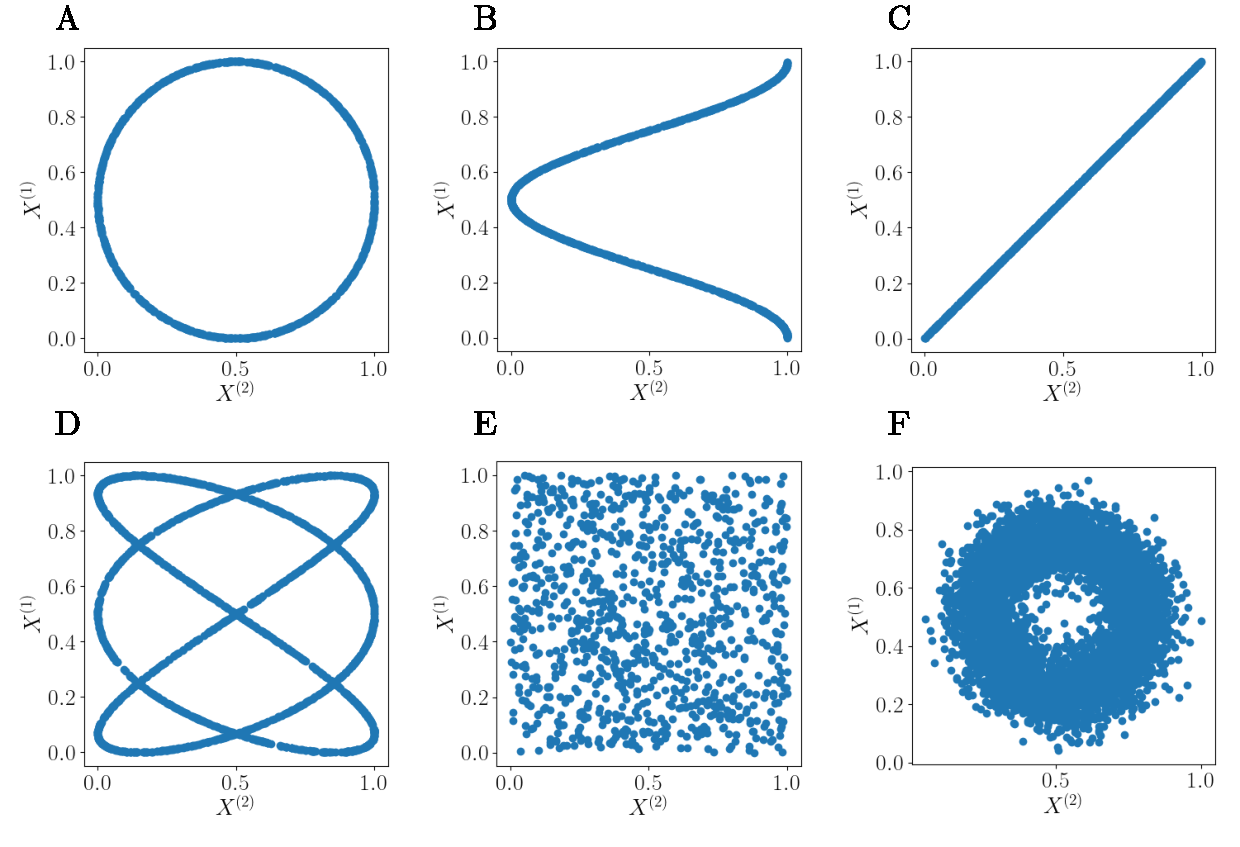
\includegraphics[width=\textwidth]{inputs/inputs.pdf}
	\caption{Dispositions d'entrées en deux dimensions étudiées dans la section suivante}
\end{figure}

\subsection{Matériel}

Les expériences présentées ici ont été réalisées en s'appuyant sur la librairie CxSOM \footnote{\url{https://github.com/HerveFrezza-Buet/cxsom}}, développée au sein de notre équipe.
Il s'agit d'une librairie C++ permettant de créer des cartes de Kohonen simples ainsi que des architectures par le modèle que nous avons présenté.
Cette librairie s'interface avec python par un module pycxsom afin de faciliter les représentations et manipulation des cartes.
Les codes C++ et python que nous avons utilisé pour générer les expériences présentées dans ce chapitre est disponible sur git : REF.
La librairie CxSOM, qui cherche à paralléliser au maximum les itérations de calcul.
Notons que la gestion du consensus passe par des mécanismes locaux aux cartes dans cette implémentation~: chaque carte envoie un signal aux cartes voisines lorsque son BMU n'est plus déplacée. Si une carte reçoit un signal de toutes ses connexions indiquant que leur BMU ne bouge plus et que son propre BMU n'est pas modifié, elle considère que le consensus est atteint.
Toutes les expériences présentées ici tournent sur un simple processeur i7.

\subsection{Méthodes}

Chaque jeu de donnée sert d'entrée d'apprentissage à une architecture de deux cartes 1D connectées réciproquement. Chaque carte a une taille fixée de 500 unités, indexées entre 0 et 1, et possède deux couches de poids $\w_e$ et $\w_c$. Les rayons de voisinage sont d'abord choisis à $r_e = 0.2$ et $r_c = 0.02$.
La génération des entrées suit le processus suivant~: $U$ est tiré uniformément dans $[0,1]$, puis les entrées $\inpx\m{1}$ et $\inpx\m{2}$ sont ensuite calculées à partir de la valeur de $U$.
L'apprentissage est réalisé sur un échantillon de 50000 itérations, générés aléatoirement. Les tests sont ensuite réalisés sur 5000 points générés aléatoirement selon la même distribution.

\section{Résultats}

Le premier but de cette étude est d'identifier des comportements \emph{systémiques} émergeant d'une architecture simple à deux et trois cartes, sur des entrées en deux et trois dimensions.
Nous avons identifié certains comportements au chapitre précédent, que nous évaluerons sur d'autres données entrées. Nous rappelons d'abord les comportements qu'on peut attendre d'une architecture de cartes.

\subsection{Entrées disposées sur un cercle : formulation d'hypothèses}

Revenons sur l'expérience précédemment présentée au chapitre \ref{chap:representation}, réalisée sur des entrées disposées selon un cercle. Nous avons alors relevé plusieurs comportements se différenciant de ce qu'on aurait pu voir avec une carte classique. Cette expérience a l'avantage d'être un cas de figure très simple d'entrées multimodales.

\subsubsection{Convergence des poids}

Dans une carte de Kohonen classique, le rayon de voisinage et le taux d'apprentissage sont décroissants au cours des itérations. Cette opération permet d'assurer un dépliement des cartes au début de l'apprentissage puis assure la convergence des poids $\w$ des cartes lorsque les paramètres décroissent.
Dans notre étude, nous choisissons de ne pas modifier les paramètres d'apprentissage au cours des itérations.
Sans chercher à démontrer mathématiquement une convergence des poids, déjà difficile à démontrer sur des cartes de Kohonen classique, nous pouvons évaluer expérimentalement la convergence des poids au cours de l'apprentissage.
La figure~\ref{fig:conv} présente l'évolution de la modification des poids $\w\ext$ et $\w\cont$ dans chaque carte au cours de l'apprentissage. La différence considérée ici est $||\w(p,t) - \w(p,t-1)||_{\infty}$ (maximum sur $p$ des différences entre les poids à l'instant $t$ et l'instant $t-1$). Ce calcul de différence est moyenné pour 10 expériences, chacune lancée sur des entrées aléatoires tirées de la même distribution sur le cercle et pour une initialisation aléatoire des poids des cartes.
Nous observons que cette courbe tend vers $0$ pour chaque courbe de poids, donc que tous les poids tendent vers une position stable.

Cette convergence est favorisée par la différence de contribution dans l'activité globale des activations externes et contextuelles, calculée, rappelons le, par~: 
$$ a_g = \sqrt{a_e \cdot (\beta a_e + (1-\beta)a_c)}$$
La carte se comporte donc principalement comme une carte de Kohonen classique apprenant sur des entrées externes, qui pour des cartes 1D sur des entrées 1D converge sans problème même en l'absence de décroissance des paramètres d'apprentissage.
La convergence est également favorisée par la différence entre rayons de voisinage externes et contextuels, qui apporte deux échelles d'apprentissage.
Notons toutefois que nous sommes sur un cas particulier de cartes 1D sur des entrées 1D.
Nous verrons que la convergence en l'absence de décroissance de paramètres pose plus de problèmes sur des cartes en deux dimensions, comme il y a plus de configurations possibles pour la carte~; mais nous verrons que pour des rayons de voisinage bien choisis, la convergence est assurée également en deux dimensions.

\begin{figure}
	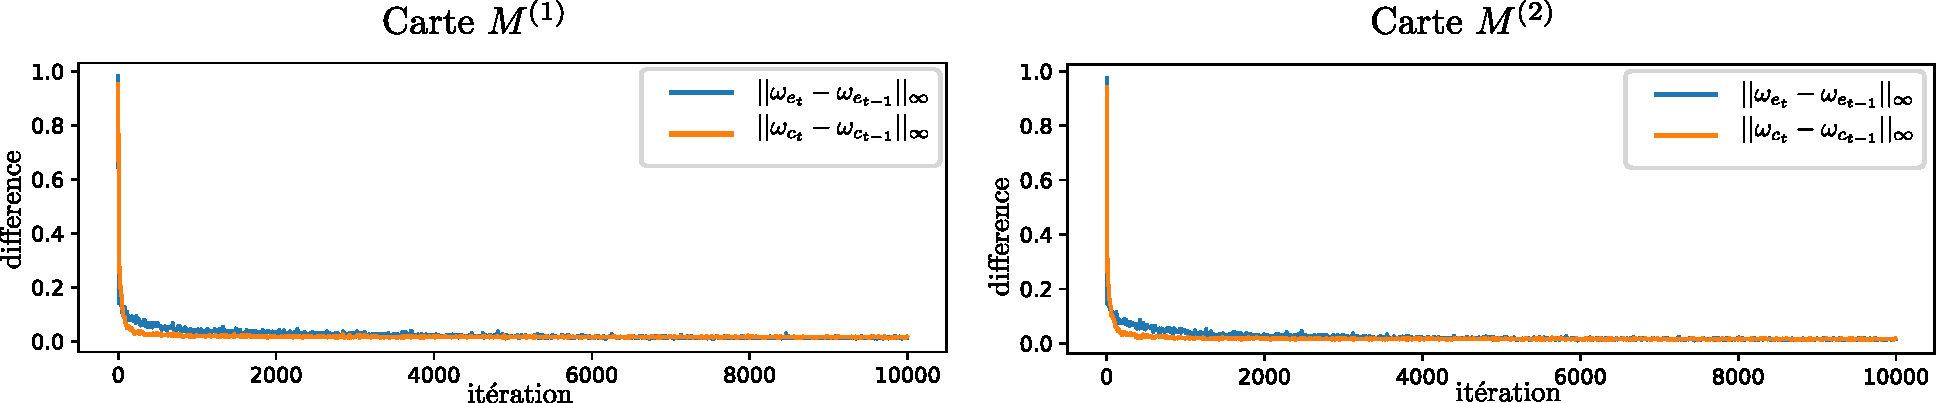
\includegraphics[width=\textwidth]{convergence/cercle_moy.pdf}
	\caption{Pour chaque carte, nous représentons l'évolution en fonction du temps d'apprentissage, de la différence maximale en valeur absolue entre les poids à l'instant $t$ et ceux à $t+1$ $\w(t)$ et $\w(t+1)$. Les entrées sont ici un cercle en deux dimensions. La différence est ici moyennée sur 10 expériences.
	Ces tracés montrent que les poids externes et contextuels convergent rapidement vers une position stable.\label{fig:conv}}
\end{figure}


\subsubsection{Disposition des poids}

Analysons d'abord la forme des poids contextuels de $M\m{1}$, tracés en figure~\ref{fig:w} sans les commenter. Les poids externes, en orange, présentent une disposition similaire à ceux observés dans la carte classique (b). Les poids contextuels, en bleu, présentent une forme de vagues. Nous ajoutons à ces deux courbes le tracé des valeur des entrées selon la position de leur BMU, en vert et rose sur la figure.

On remarque d'abord que les positions dans la carte $M\m{1}$ se répartissent en zones de BMUs, séparées par des zones mortes dans lesquelles aucune entrée n'a gagné. 
C'est une première différence avec une carte classique, pour laquelle toutes les positions seront BMUs lorsque les entrées sont distribuées de façon continue.


Les zones dans lesquelles il y a des BMUs correspondent aux extremum des poids contextuels et leurs alentours. C'est un phénomène inhabituel pour une carte de Kohonen. 
Les entrées $\inpx\m{1}$, dans la carte classique (b), correspondent à la courbe de poids externe: la valeur du poids du gagnant est toujours très proche de la valeur de l'entrée. Dans la carte $M\m{1}$, les entrées externes $\inpx\m{1}$ orange sont proches de la courbe de poids externes, mais avec plus d'erreur de quantification.
Les deux points rouge et bleu ayant la même valeur de $x$ ont un BMU différent dans la carte $M\m{1}$, alors que ces deux échantillons ont le même BMU dans la carte apprenant indépendamment sur les valeurs de $x$. Ainsi, la carte connectée au sein de CxSOM différencie les échantillons en fonction de non seulement leur entrée externe, mais aussi de l'entrée de l'autre carte de l'architecture. La plage de valeurs des $\inpx\m{1}$ gagnant dans un des zones recoupe les plages de valeurs gagnant dans les zones situées à gauche et à droite. Par exemple, la zone dans laquelle l'échantillon rouge gagne, autour de $\bmu\m{1} = 0.25$. La partie des entrées située en dessous de la courbe de poids externe recoupe les valeurs d'entrées gagnant dans la zone précédente; la partie située au dessous de la courbe de poids externe recoupe des valeurs gagnant dans la partie suivante. Pour une entrée externe, le choix de la zone de BMU dans laquelle elle gagnera dépend alors de l'entrée contextuelle. 


Dans la carte $M\m{1}$, une unité se spécialise donc par rapport aux deux entrées et non pas une seule comme dans la carte indépendante~: les entrées externes et l'entrée contextuelles. C'est bien ce à quoi on s'attendait en ayant deux couches de poids. Ce qui est intéressant est que cette différenciation est réalisée par la répartition des unités en un nombre fini de zones distinctes. Dans chaque zone, les unités sont BMUs pour un segment de valeurs d'entrée externe et contextuelles. Au sein d'une zone, la répartition des entrées externe selon le BMUs est ordonnée, comme ce serait le cas dans une carte auto-organisatrice classique. Le comportement de la carte au sein d'une zone reste donc similaire à celui d'une carte classique.

Deux zones adjacentes correspondent par ailleurs à des segments de valeur d'entrée en partie superposés, et des segments de valeurs d'entrées contextuelles différentes. Il s'agit d'une deuxième échelle d'organisation, qui garde également l'aspect ordonné d'une carte classique. Ces zones sont créées par auto-organisation~; aucun paramètre de la carte n'a été modifié pendant l'apprentissage pour former ces zones, et le nombre d'unités allouées par auto-organisation dans chaque zone est à peu près égal. La carte agit un peu comme une base de données structurée avec des indices primaires et des indices secondaires pour chaque neurone, l'indice primaire étant la zone de la carte, et l'indice secondaire la position dans cette zone.

Les résultats de cette expérience nous permettent donc de formuler les hypothèses suivantes concernant le comportement de cartes en une dimension~:

\begin{itemize}
	\item Les poids externes de chacune des cartes effectuent une quantification vectorielle correcte sur leurs entrées externe \ref{fig:qv}
	\item Les poids contextuels de chaque carte s'organisent en zones distinctes. Une zone correspond à un même intervalle de valeur pour $\inpx$ et $U$. Deux zones adjacentes encodent le même intervalle de valeurs pour $X$ mais des valeurs distinctes de $U$. \ref{fig:w} Ces zones se caractérisent par un étirement de la carte entre deux valeurs éloignées, apportant un aspect discontinu. Cette discontinuité passe en fait par la présence d'une zone peu dense de la carte contenant des n\oe{}uds qui ne seront jamais BMUs \ref{fig:w_zoom}. Nous verrons en section Prédiction que la formation de ces zones permet à la carte de prendre des décisions lors d'une phase de prédiction, ce qui n'est pas le cas autrement.
	\item La séparation des $U$ peut être vérifiée par une relation fonctionnelle entre $U$ et $\bmu$ dans chaque carte.
\end{itemize}

Nous chercherons à vérifier toutes ces observations sur d'autres dispositions d'entrées dans des structures de deux cartes, et nous nous demanderons si la création de zones dépend de la disposition des entrées~: une valeur de $X\m{1}$ correspondant à 1 valeur de $\inpx\m{2}$ dans la distribution identité, 2 valeur dans la distribution en cercle, plusieurs pour les courbes de lissajou, et enfin une infinité de valeurs lorsque les deux entrées sont indépendantes (carré $[0,1]^2$). 
Nous chercherons donc à savoir comment ces zones sont construites. Enfin, une caractéristique d'une carte de Kohonen est sa robustesse au bruit. Nous vérifierons si cette propriété se traduit également dans les architectures de deux cartes.

Nous étendrons ensuite notre étude aux structures de trois cartes apprenant sur trois entrées 1D connectées par un $U$ 1D. De cette manière, la connaissance de deux entrées et du modèle de relation nous permet de déduire la troisième entrée. Nous montrerons que cette tâche de prédiction est également effectuée par une architecture de trois cartes. Cette tâche de prédiction apparait comme une preuve expérimentale de l'apprentissage du modèle.
Nous pourrons enfin observer le comportement des cartes lorsqu'elles reçoivent plus d'une connexion contextuelle.

\begin{figure}
	\centering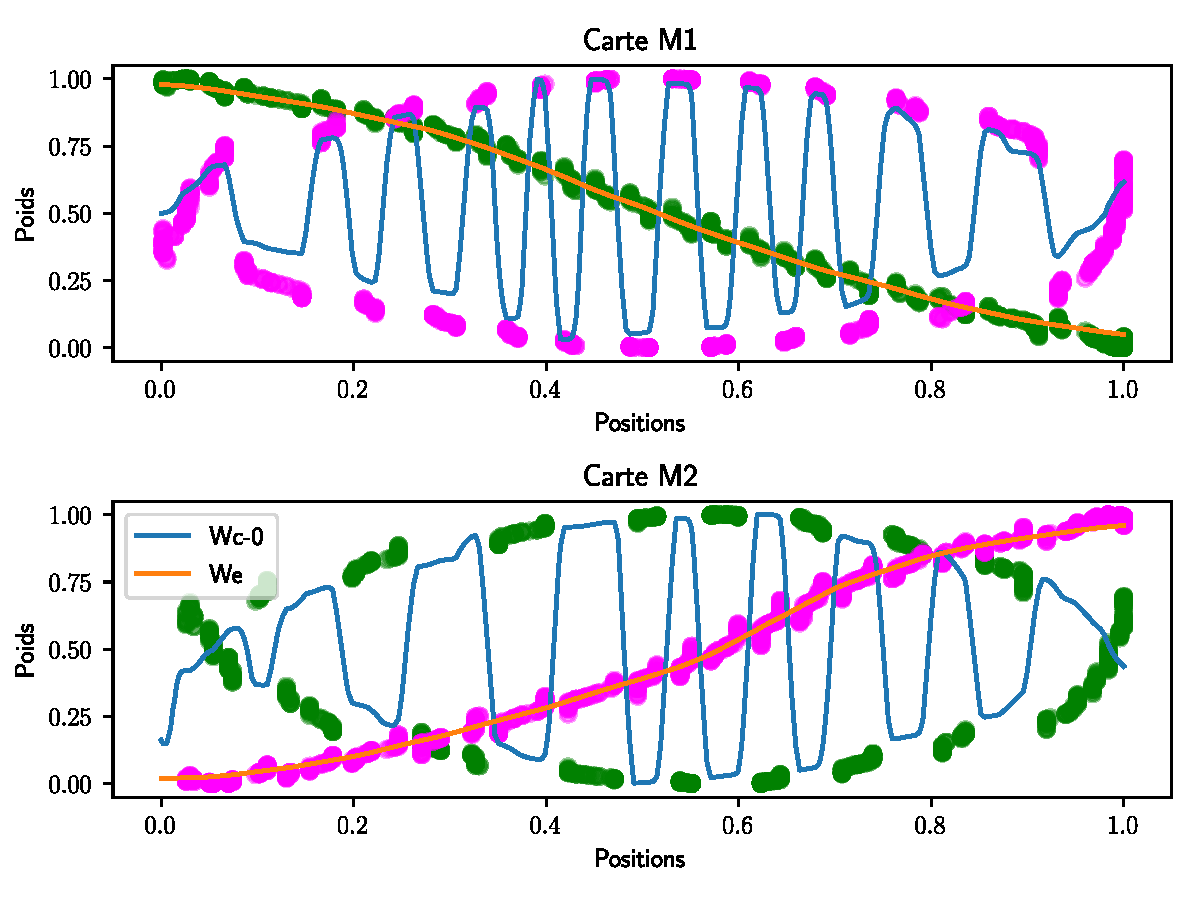
\includegraphics[width=0.9\textwidth]{2som_cercle_w.pdf}
	\caption{Représentation cartographique des poids et entrées lors d'une phase de test selon la position dans chacune des cartes. Nous remarquons que les poids d'une carte, par exemple la carte $M^{(1)}$ s'organisent en zones différenciant les valeurs de la paire $X^{(1)}, X^{(2)}$ et non seulement de la valeur de $X^{(1)}$. Deux zones adjacentes codent pour des valeurs de $X^{(1)}$ proches, mais $X^{(2)}$ différents. Au sein d'une même zone, les BMUs s'organisent sous la forme d'une mini carte sur les valeurs de l'entrée contextuelle. Ces zones se forment de manière auto-organisée. \label{fig:w}}
\end{figure}

\begin{figure}
	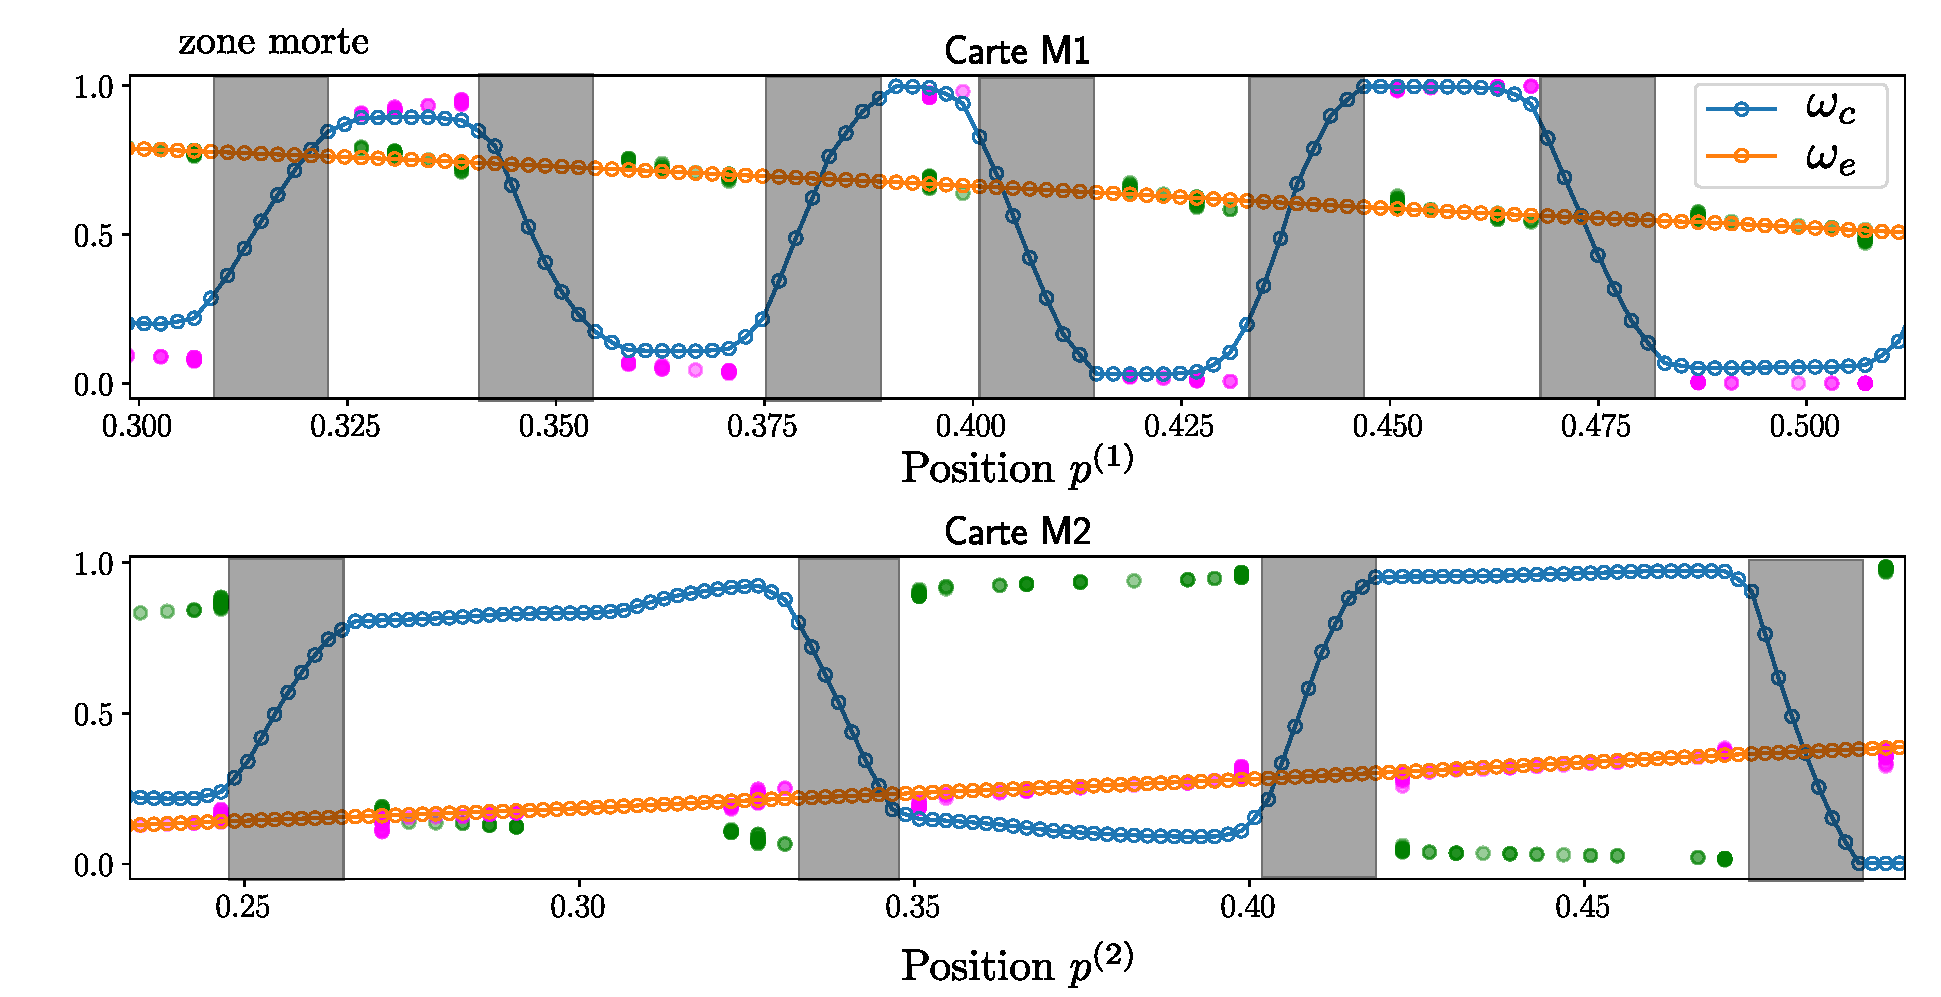
\includegraphics[width=\textwidth]{2som_cercle_w_zoom_with_nodes.pdf}
	\caption{Zoom sur la figure \ref{fig:w}. Nous y faisons apparaître la position sur la courbe des noeuds de la carte. Nous voyons que les zones grisées contiennent quelques n\oe{}uds qui ne sont jamais BMUsé; ce sont des zones mortes. Nous en concluons que la discontinuité introduite par la formation de zones est une "fausse" discontinuité et se produit en reliant des valeur de $\w_c$ éloignée en étirant une portion de carte morte. \label{fig:w_zoom}}
\end{figure}

\begin{figure}
	\centering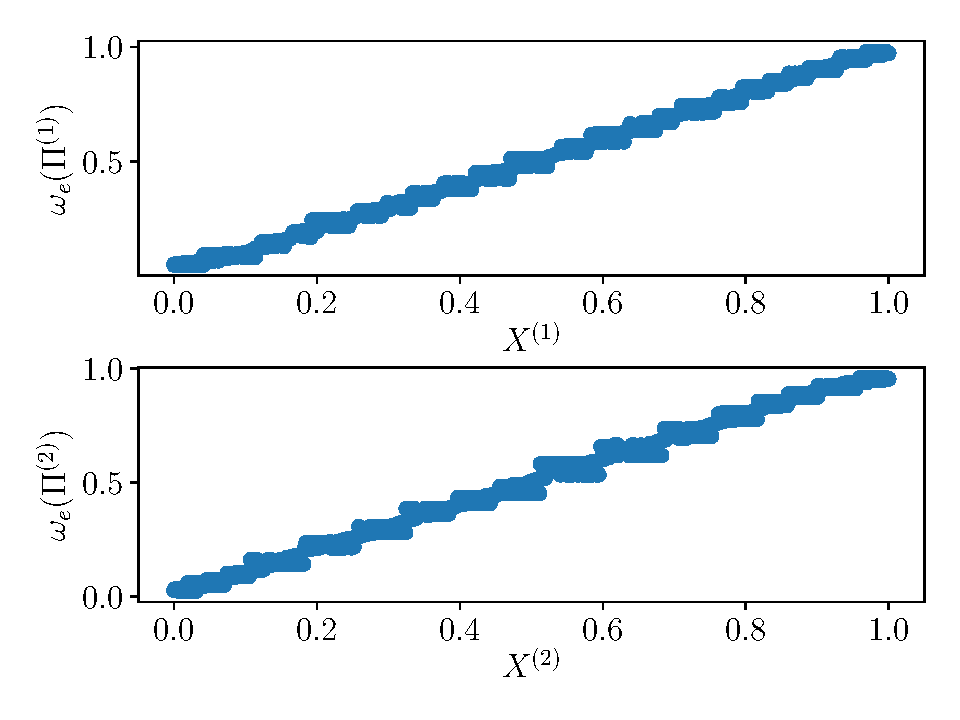
\includegraphics[width=0.8\textwidth]{2som_cercle_err.pdf}
	\caption{Représentation de l'erreur de quantification sur les valeurs de $X^{(1)}$ et $X^{(2)}$. Le poids externe du BMU est proche de la valeur de l'entrée~; chaque carte possède donc une capacité de quantification vectorielle sur ses entrées. \label{fig:qv}}
\end{figure}

% \begin{figure}
% 	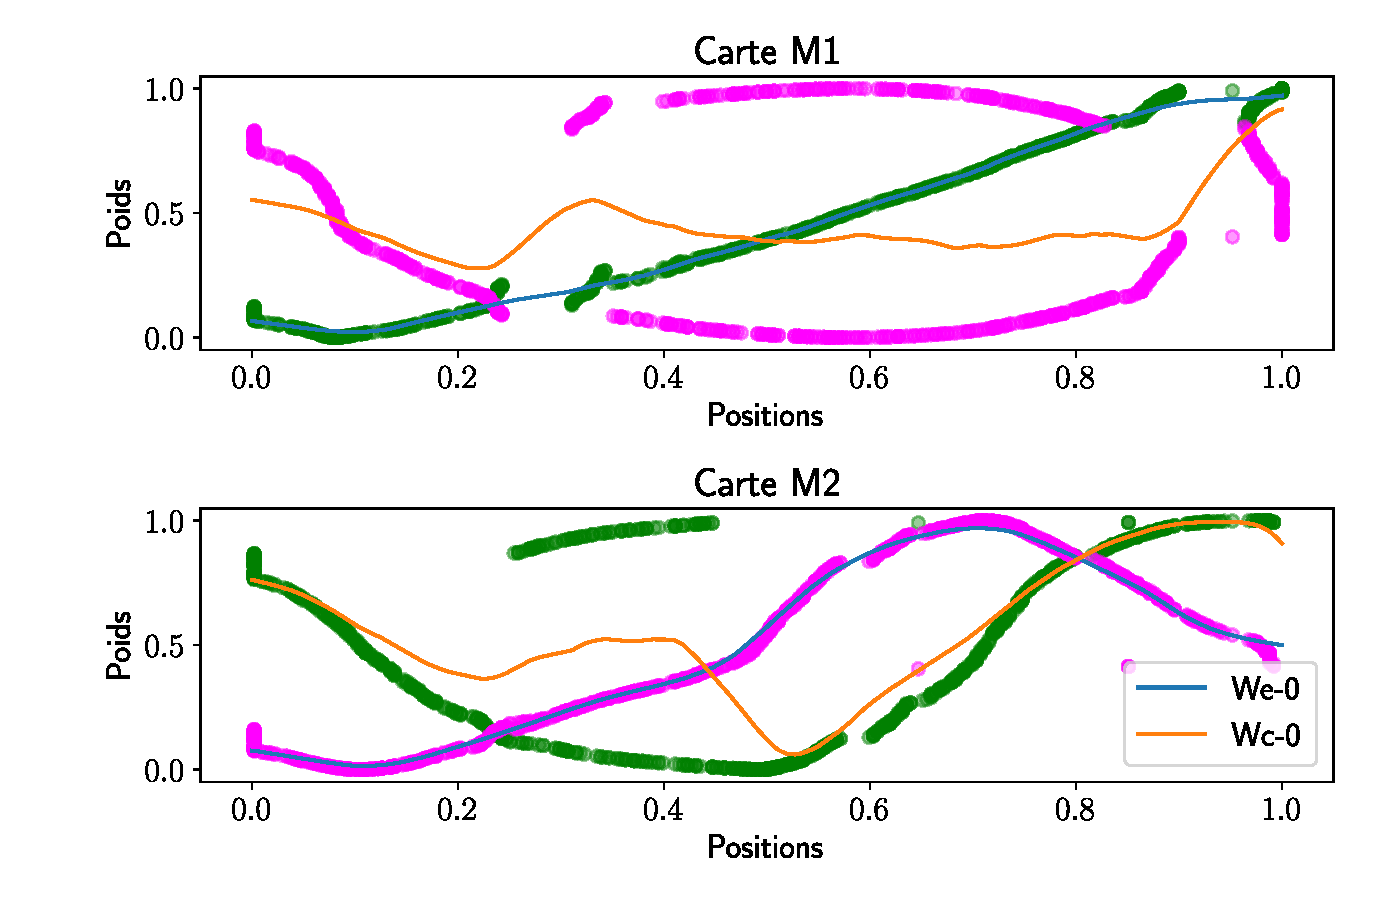
\includegraphics[width=\textwidth]{weights_rcre.pdf}
% 	\caption{Représentation cartographique des poids de la carte lorsque $r_c = r_e = 0.1$. La présence de zones n'est pas observée.}
% \end{figure}

\subsection{Vérification des hypothèses sur différentes distributions d'entrées}

La figure \ref{fig:id_results} présente la disposition des poids et entrées des cartes lorsque $\inpx\m{1}$ et $\inpx\m{2}$ sont identiques. Les poids externes et contextuels ne forment pas de zones et les deux cartes se comportent comme une seule carte simple sur $\inpx\m{1} = \inpx\m{2}$
En figure~\ref{fig:cos_results}, la dépendance entre les entrées n'est plus bijective. $\inpx\m{2}$ est fonction de $\inpx\m{1}$~; de ce fait, la carte $M\m{1}$ ne forme pas de zones. Au contraire, la carte $M\m{2}$ doit a présent se diviser pour apprendre les deux valeurs de $\bmu\m{1}$ possibles correspondant à $\inpx\m{2}$. Ces expériences montrent que la formation de zones est bien déterminée par la disposition des entrées.

\begin{figure}
	\centering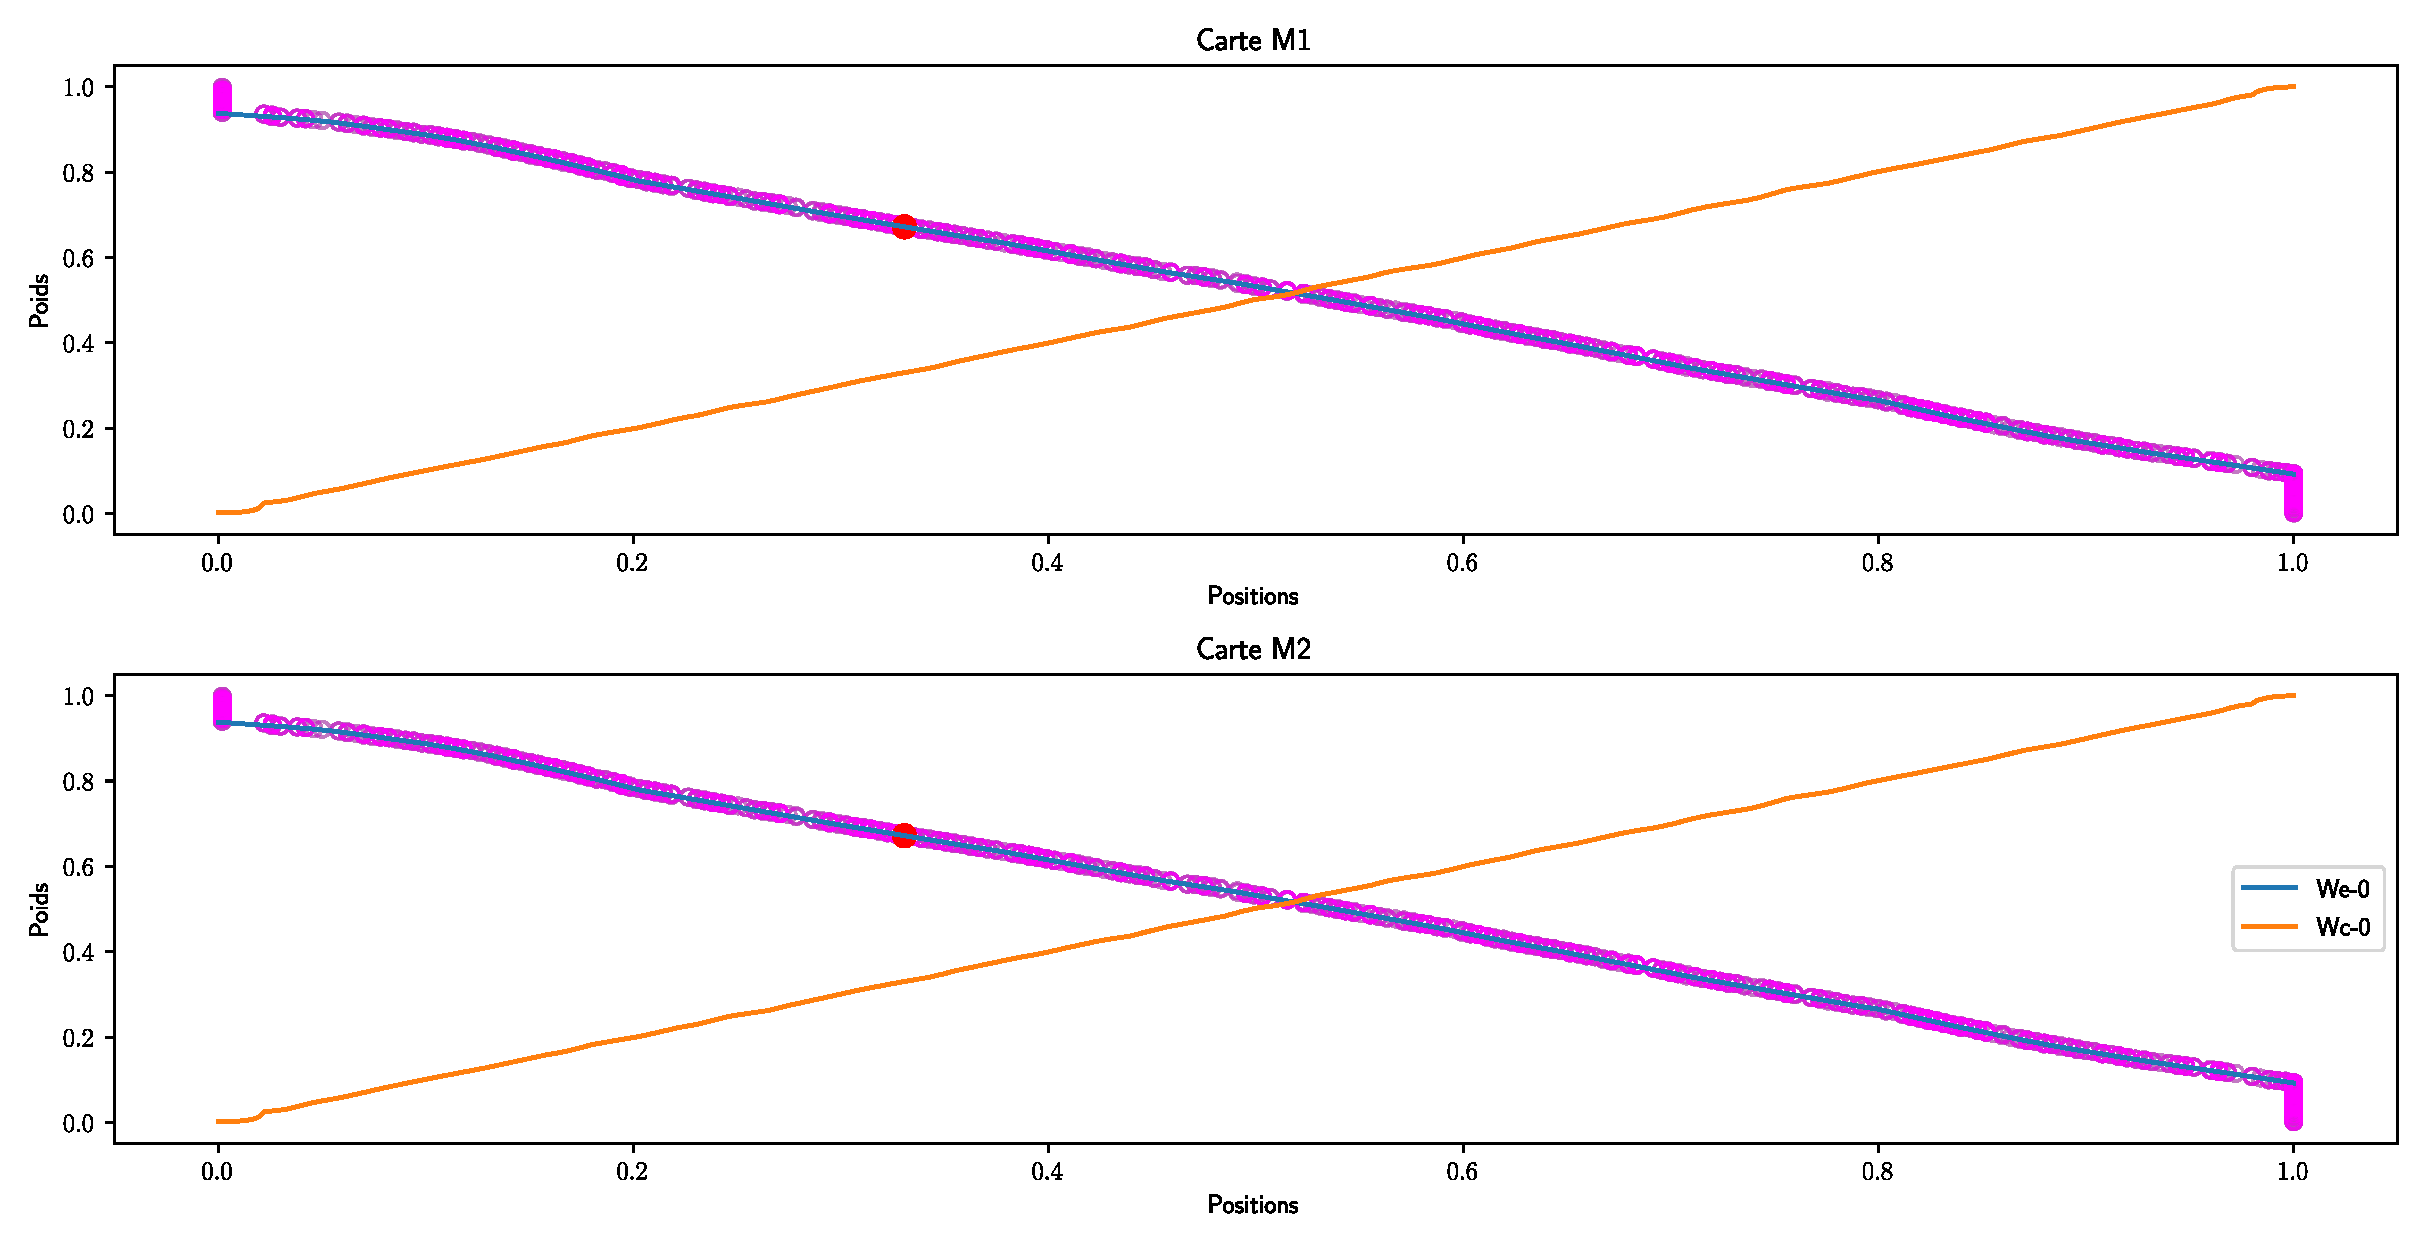
\includegraphics[width=0.6\textwidth]{2som_id_w.pdf}
	\caption{Représentation cartographique des poids et entrées pour la disposition identité. Les poids externes et contextuels sont superposés, et les poids contextuels n'ont pas besoin de former de zones \label{fig:id_results}}
	\end{figure}
	
	\begin{figure}
		\centering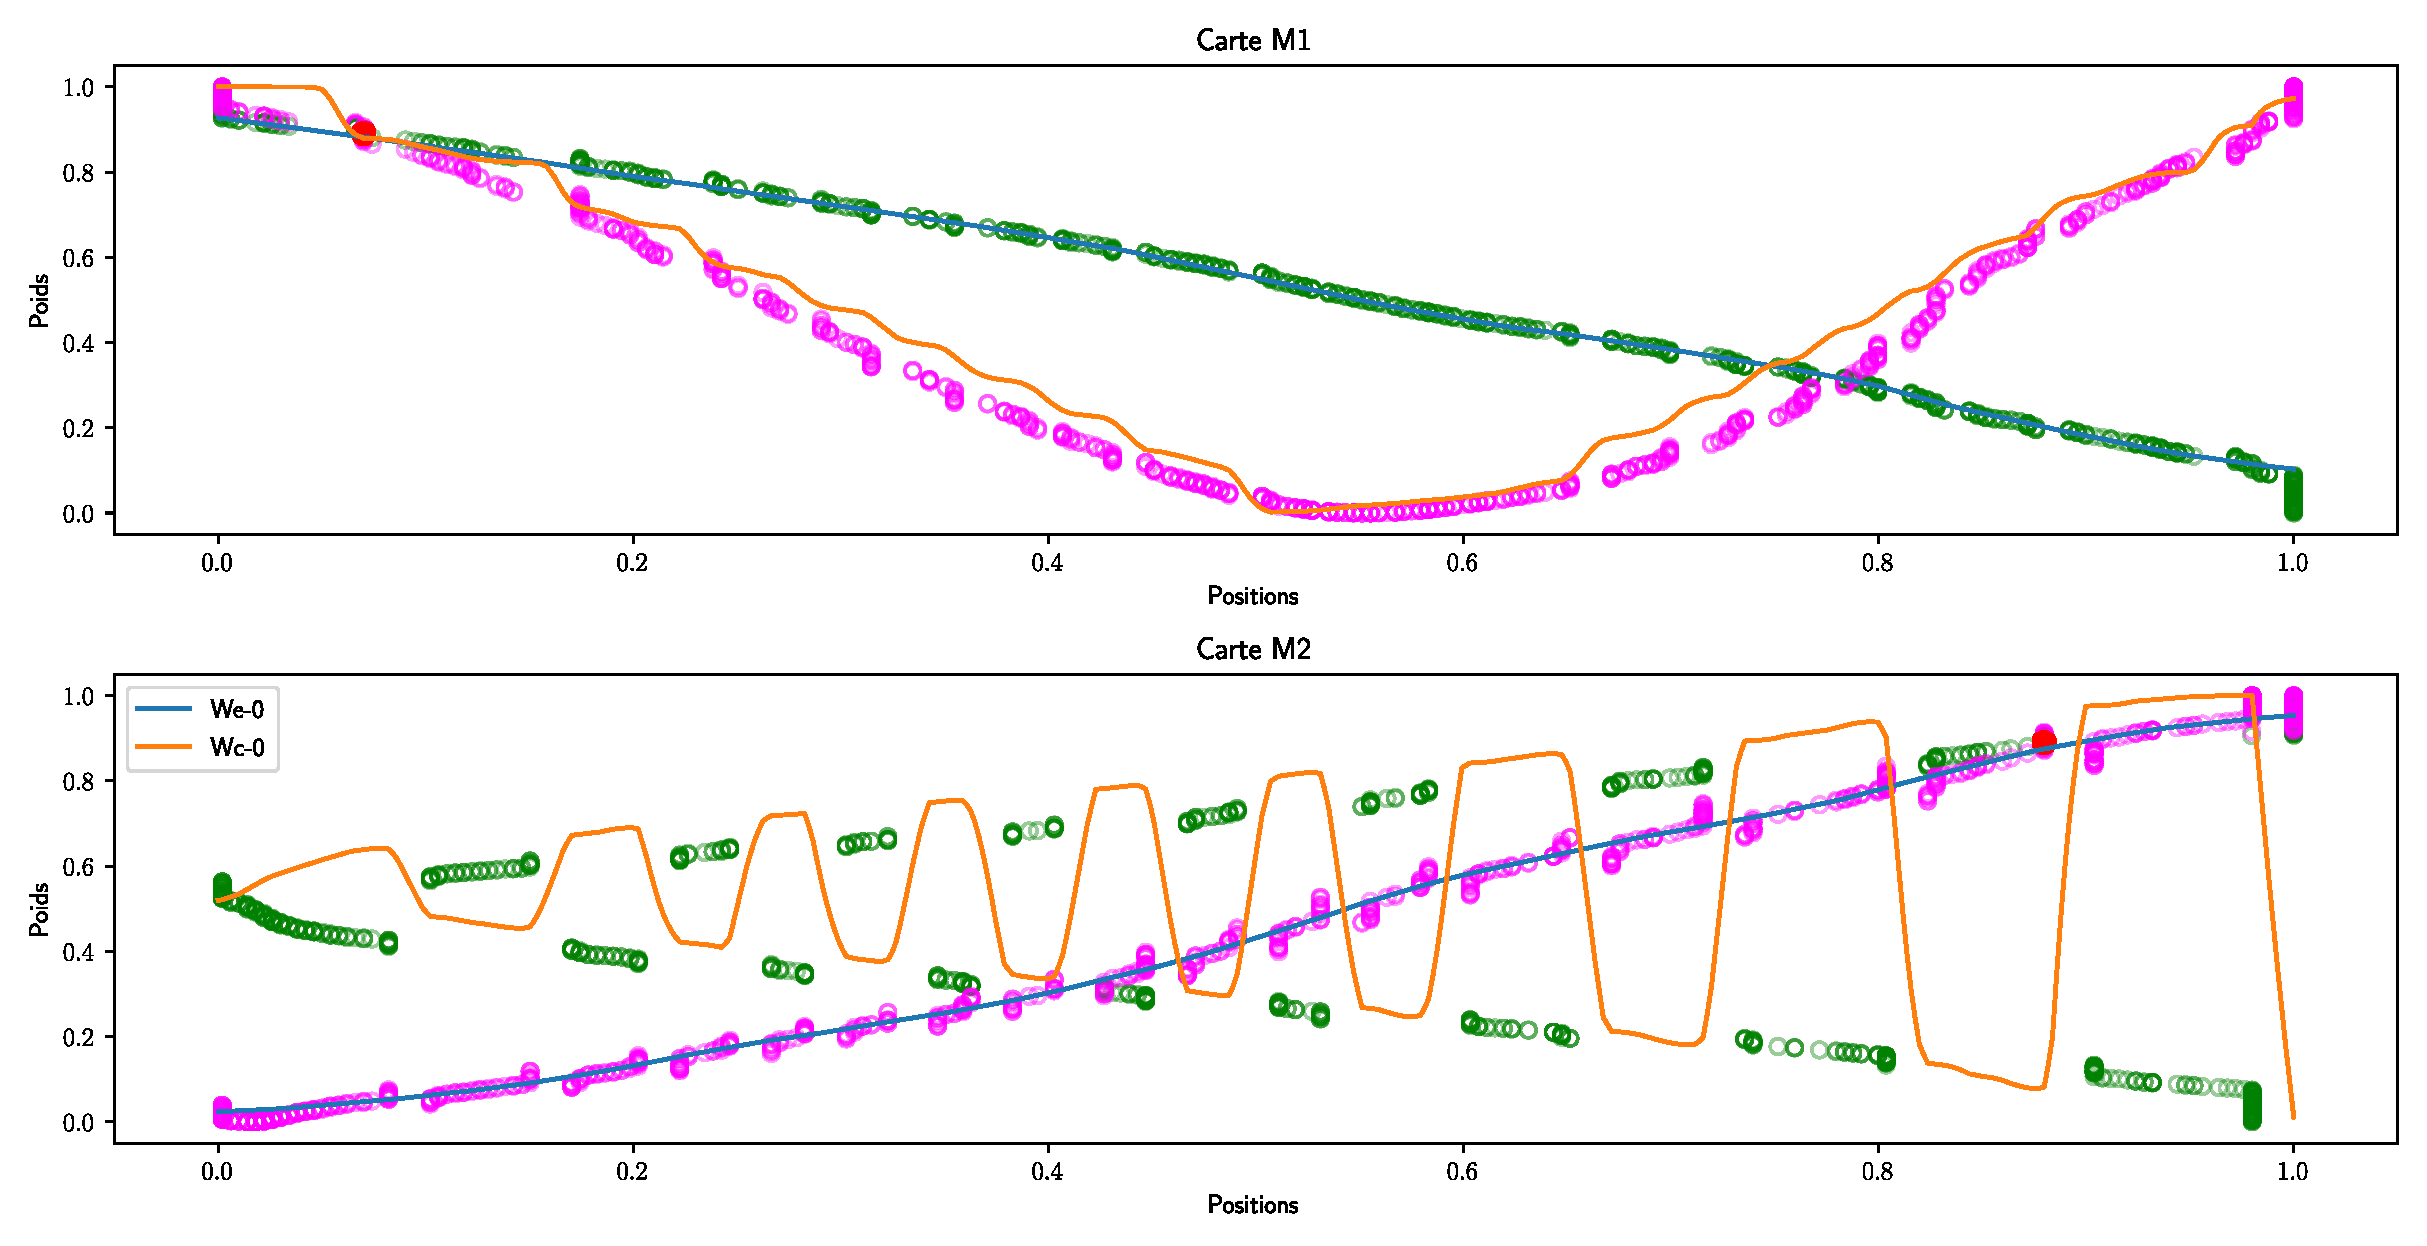
\includegraphics[width=0.6\textwidth]{2som_cos_w.pdf}
		\caption{Représentation cartographique des poids et entrées pour $\inpx\m{2} = cos(\inpx\m{1}$. Les poids contextuels de la carte $M\m{1}$ ne forment pas de zones car une seule valeur de $\inpx\m{2}$ correspond à une entrée $\inpx\m{1}$. Au contraire, les poids de la carte $M\m{2}$ s'organisent pour gérer la distinction. \label{fig:cos_results}}
	\end{figure}

La couche de poids externe converge plus vite que la couche contextuelle par la différence entre rayons de voisinage. De ce fait, les positions du BMU respectent les relations de distances dans l'espace d'entrée externe~: deux points éloignés sur $\w_e$ ont des poids éloignés.

Si le nombre de valeurs possibles pour $\inpx\m{2}$ pour une même valeur de $\inpx\m{1}$ augmente, on peut supposer que la carte continuera à s'organiser en zones.
La figure \ref{fig:lissa} présente l'organisation obtenue pour des points placés sur une courbe de lissajous, dans laquelle une valeur de $X\m{1}$ correspond à 4 à 6 valeurs de $\inpx\m{2}$ et inversement. Enfin, la figure~\ref{fig:ind} présente l'organisation obtenue lorsque les points sont dans le carré $[0,1]^2$: les entrées sont indépendantes.

Dans ces deux derniers cas, les cartes présentent une organisation en zones des poids contextuels, tout comme le comportement observé sur le cercle. 
Ainsi, nous pouvons conclure que la présence de zones en tant que telle est donc un comportement systématique de la carte étant donné qu'elles sont observées même lorsque les entrées sont indépendantes. Par contre, la forme des zones dépend de la relation entre entrée.

Sur la distribution indépendante, contrairement au cercle, la carte ne présente pas de zone morte. La totalité d'une zone se déploie de manière à couvrir l'ensemble des valeurs de $U$, ce qui est également observé en figure ~\ref{fig:lissa} pour les courbes de Lissajous. 
Une zone agit alors comme une petite carte d'une sous-région de l'espace d'entrée. La figure 

Nous avons remarqué que les poids externes se déplient en priorité et respectent les distances~: deux n\oe{}uds distants dans la carte ont des poids distants et gagnent pour des entrées distantes.  
Par contre, nous remarquons que deux n\oe{}uds proches peuvent gagner pour une même valeur d'entrée externe, bien qu'ayant une valeur de poids contextuel légèrement différente.
L'intervalle de valeurs d'entrées codées au sein de deux zones adjacentes se recouvrent.

Les deux cartes de Kohonen se comportent donc pour paver l'espace d'entrée différemment, et définissent un compromis entre qualité de l'approximation de l'entrée externe par $\w_e(\bmu)$ et différenciation des BMUs selon le modèle d'entrée complet $U$.


\begin{figure}
	\centering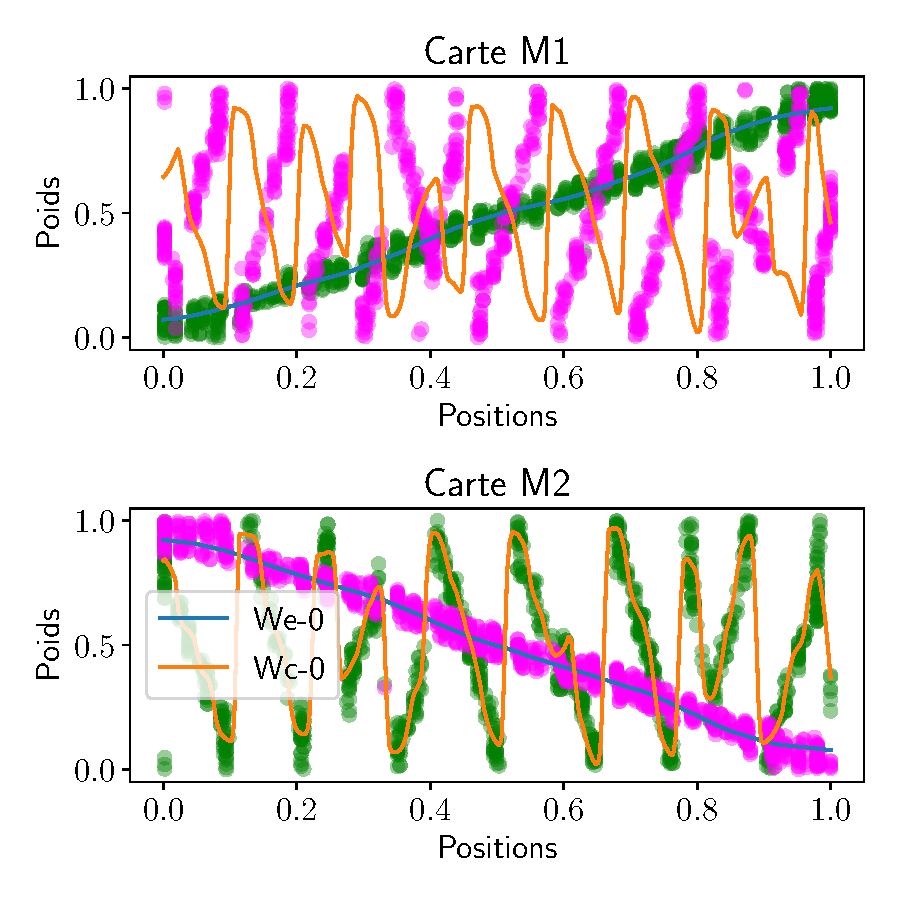
\includegraphics[width=0.6\textwidth]{2som_square_w.pdf}
	\caption{Représentation cartographique des poids et entrées pour la disposition carré}
\end{figure}

\begin{figure}
	\centering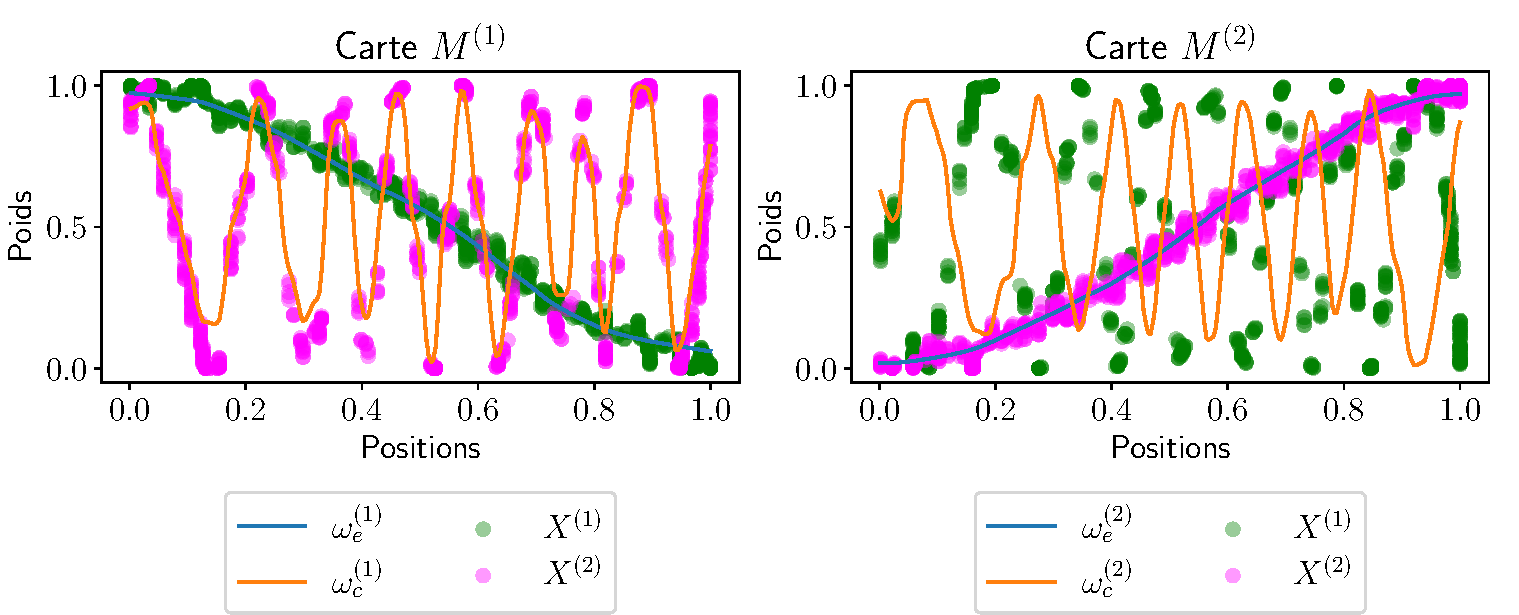
\includegraphics[width=0.6\textwidth]{lissa/weights_19999.pdf}
	\caption{Représentation cartographique des poids et entrées pour des entrées sur une courbe de Lissajous. Les poids contextuels continuent de former des zones.}
\end{figure}

\begin{figure}
	\begin{minipage}{0.48\textwidth}
		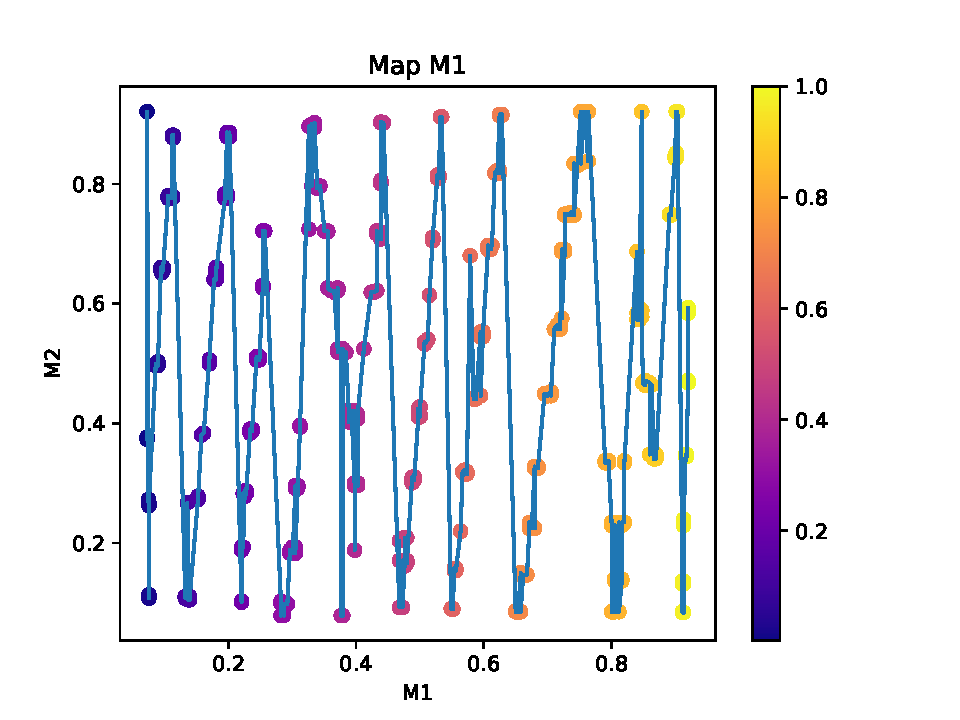
\includegraphics[width=\textwidth]{2som_square_d}
	\end{minipage}
	\begin{minipage}{0.48\textwidth}
		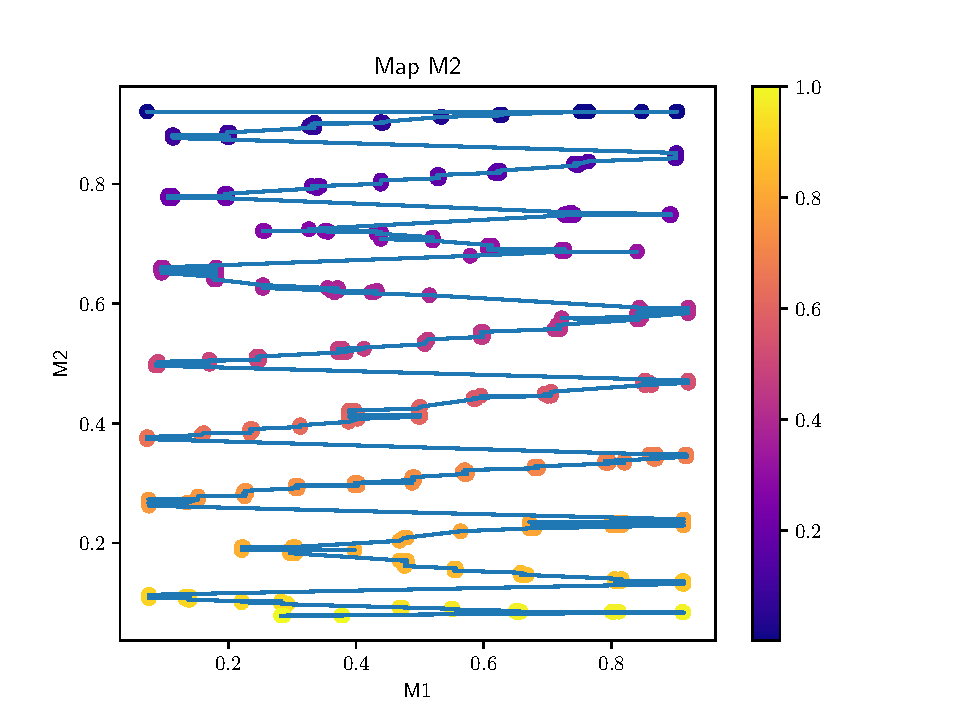
\includegraphics[width=\textwidth]{2som_square_d2}
	\end{minipage}
	\caption{Représentation de la distortion des poids des deux cartes dans l'espace d'entrée $\inpx\m{1}, \inpx\m{2}$ lorsque les entrées sont indépendantes. Les cartes s'organisent de façon à quadriller le carré, l'une selon les $\inpx\m{1}$, l'autre selon les $\inpx\m{2}$. Bien que chaque carte aie 500 noeuds, on observe seulement environ 90 valeurs possibles pour les paires $\w_e(\bmu\m{1}),\w_e(\bmu\m{2})$ \label{2som_p_d}}
\end{figure}

\subsection{Discussion}

Nous avons observé sur ces quelques distributions les comportements suivants~:
\begin{itemize}
	\item quantification vectorielle correctement réalisée pour chaque type d'entrée
	\item Organisation en zones dès que besoin de découpler deux valeurs de U
	\item Le comportement traduit l'existence de plusieurs valeurs de U pour une même entrée, sans forcément qu'une relation existe. Dans tous les cas, la carte effectue un découpage selon U.
	\item Lorsque relation il y a, ce découpage permettra de faire de la prédiction.
\end{itemize}

La disposition des cartes repose complètement sur les zones formées par les poids contextuels. Ces zones apparaissent grâce au fait que la proximité des poids externe est priorisé par rapport au poids contextuels par le rayon de voisinage externe 10 fois plus élevé. Ce rapport introduit une relation subordonnée entre les poids. 
Au sein d'une même zone, dans laquelle les poids externes ont des valeurs très proches, les poids contextuels s'organisent de manière à former une petite carte sur toutes les valeurs possible de l'entrée contextuelle.
On pourrait donc introduire une notion d'indices primaire et secondaire, l'indice primaire étant celui de la zone et l'indice secondaire la position dans la zone.
% Ce type d'indexation est courant dans des systèmes informatiques comme les bases de données.
Cette notion d'indices primaires et secondaires est également observée dans le cerveau, proposé en 1986 par \cite{ballard_cortical_1986}. Les neurones du cortex V1, par exemple, gèrent leurs connexions et leur organisation comme schématisé en figure~\ref{fig:ballard}.
Les neurones situés à différents emplacements sur cortex V1 ne reçoivent pas la même partie de l'entrée visuelle. Ces entrées différenciées forment une indexation~\emph{primaire} de V1. Au sein d'une zone de même indice primaire, les neurones s'organisent de façon à représenter toutes le sous espace d'entrée ayant été présenté à la zone. Cette sous-carte définit alors des indices secondaires.
%ci, la même entrée est certes présentée à toute la carte, mais l'activité externe agit comme un masque 

Le comportement des cartes jointes introduit un phénomène de discontinuité dans les poids contextuels. Cette discontinuité est en fait une fausse discontinuité puisque des zones mortes comptant 4-5 n\oe{}uds séparent séparent deux zones de poids contextuels.
On observe que plus on a de valeurs possibles pour $\inpx\m{2}$ pour une même valeur de $\inpx\m{1}$, moins on aura de n\oe{}uds morts dans les zones de discontinuité, comme le montre l'exemple du carré dans lequel il n'y a pas de n\oe{}uds morts entre zones.
Les zones sont à peu près réparties équitablement sur la cartes.
La présence de zones auto-organisées permet au cartes d'acquérir une capacité de prise de décision, que nous explorons dans la section suivante.
En effet, si une carte ne possède pas d'entrée externe, elle peut être activée par les connexions contextuelles et possède un BMU. Ce BMU peut être considéré comme une prise de décision d'une carte de l'architecture. Nous verrons que cette disposition en zones permet effectivement de 

Ces architectures de quelques cartes sont des architectures \emph{élémentaires}: toute architecture comportant plus de cartes pourra être construite à partir de petits modules. 
\begin{figure}
	\centering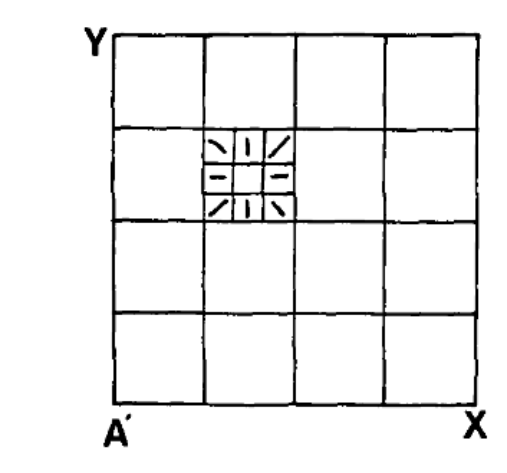
\includegraphics[width=0.5\textwidth]{ballard_primary_secondary.png}
	\caption{Schéma d'une répartition en indices primaires et secondaire des neurones d'une aire corticale présentée en \cite{ballard_cortical_1986}. Les auteurs observent que sur une carte rétinotopique des neurones, c'est à dire tracées en fonction de la position des neurones sur le cortex, la réponse de neurones est organisée en zones, les indices primaires, recevant en connexion différentes portions de l'espace d'entrée. Au sein d'une même zone, les neurones cartographient toutes les valeurs possibles de l'entrée sous forme de carte topologiquement ordonnée, formant des indices secondaires.\label{fig:ballard}}
\end{figure}

\subsection{Limites possibles}

\begin{figure}
	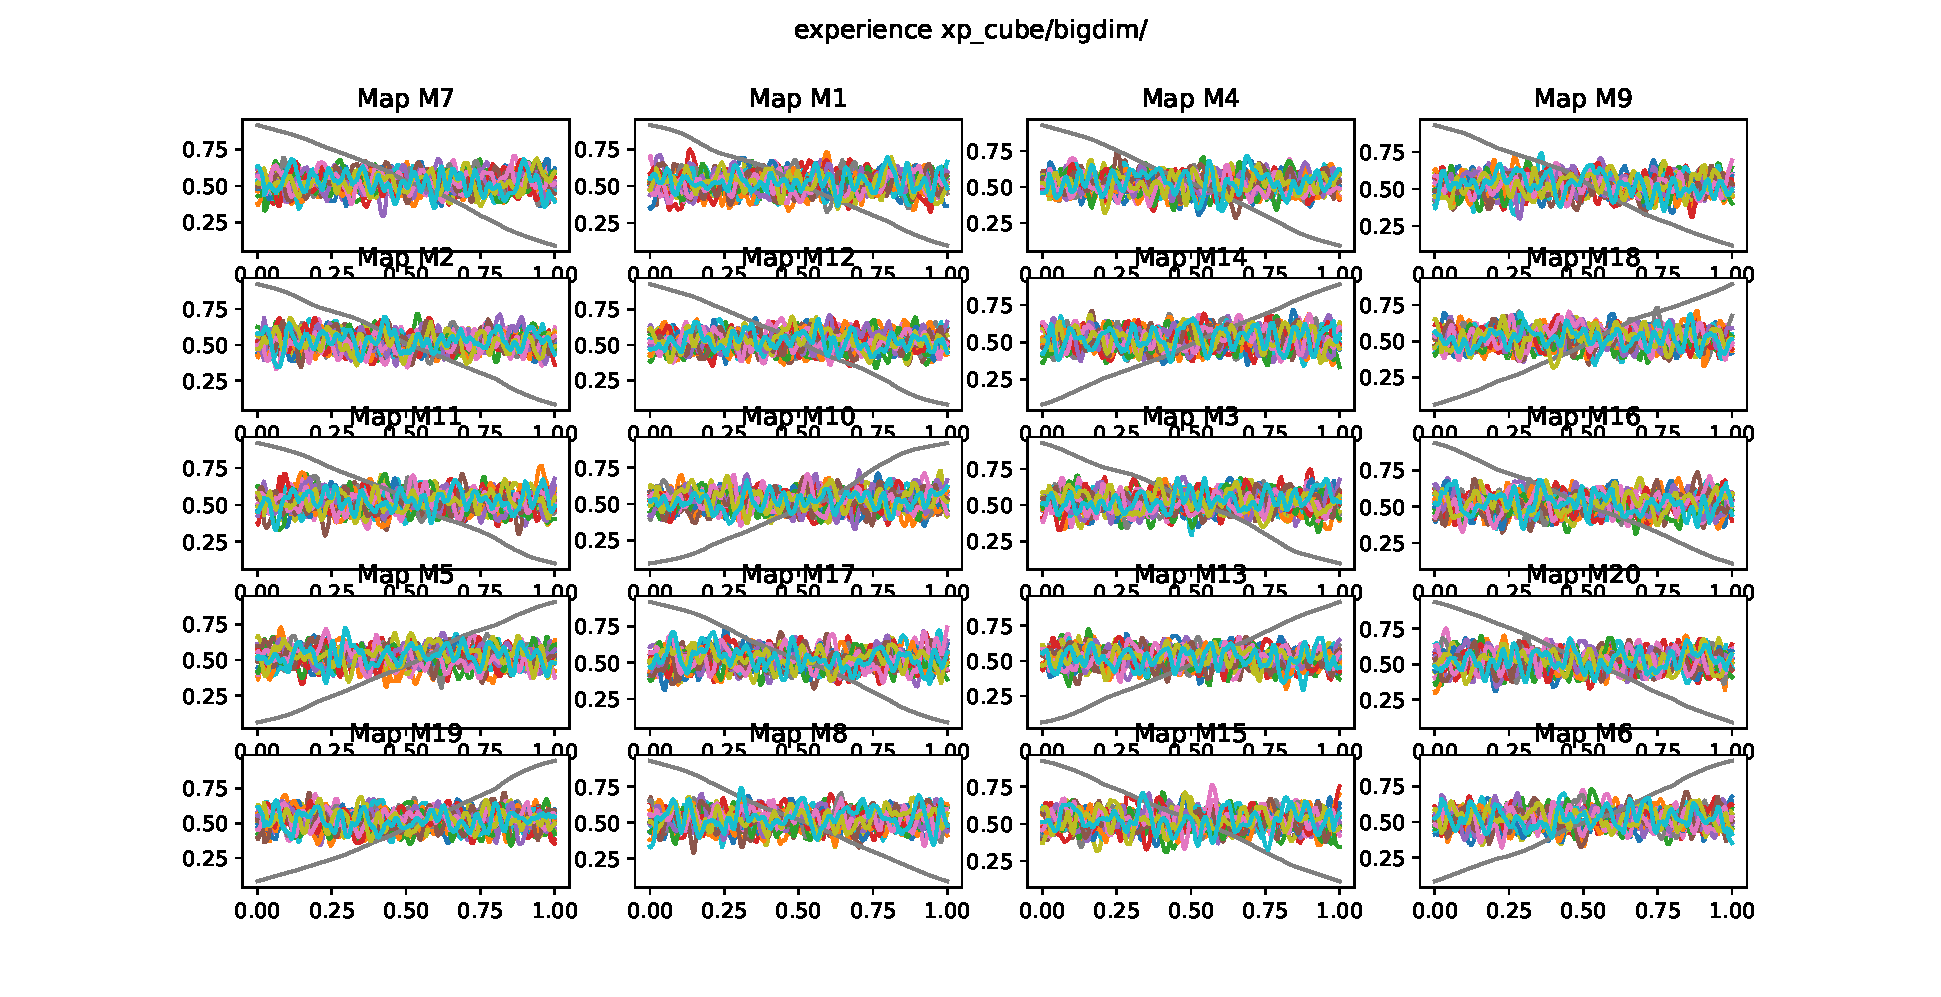
\includegraphics[width=\textwidth]{xp_cube_bigdim.pdf}
	\caption{Tracé des poids des cartes pour une architectures de 10 cartes toutes connectées. Les entrées sont ici indépendantes. Nous remarquons que les poids contextuels se moyennent autour de 0.5.}
\end{figure}
%tracé pour les valeurs sur le cercl

\section{Prédiction d'entrée}

L'observation des mécanismes d'organisation occurrant dans des architectures de deux cartes nous a confirmé que le modèle d'entrées, défini par la variable cachée, est appris dans chacune des cartes de l'architecture grâce aux connexions entre cartes.
Nous utilisons maintenant le fait qu'une architecture ait appris le modèle dans une tâche de prédiction d'entrée.

Cette utilisation en tant que prédiction a certes une valeur applicative, car il s'agit d'un cas d'utilisation possible d'une architecture CxSOM pour une tâche de mémoire associative. Néanmoins, la prédiction permet avant tout de valider l'apprentissage du modèle par l'architecture d'un point de vue d'une carte. Par exemple, dans le cas de données réelles, le modèle d'entrée n'est pas forcément connu. La prédiction permet alors de valider l'apprentissage du modèle.

Rappelons la structure utilisée pour la tâche de prédiction (voir figure~\ref{fig:schema_pred})~: après l'apprentissage de l'architecture sur l'ensemble des entrées, nous choisissons une des cartes comme carte prédictive. 
Lors de la phase de prédiction, cette carte ne reçoit plus d'entrée externe, mais seulement les entrées contextuelles venant des autres cartes de l'architecture. 
Les autres cartes reçoivent quant à elles toujours leurs entrées externes et contextuelles. La phase de prédiction est une phase de test durant laquelle les poids de toutes les cartes ne sont pas mis à jour. Les règles de calcul et paramètres sont conservés entre apprentissage et prédiction. La carte ne recevant pas d'entrée externe prend simplement comme activité globale son activité contextuelle. 

\begin{figure}
	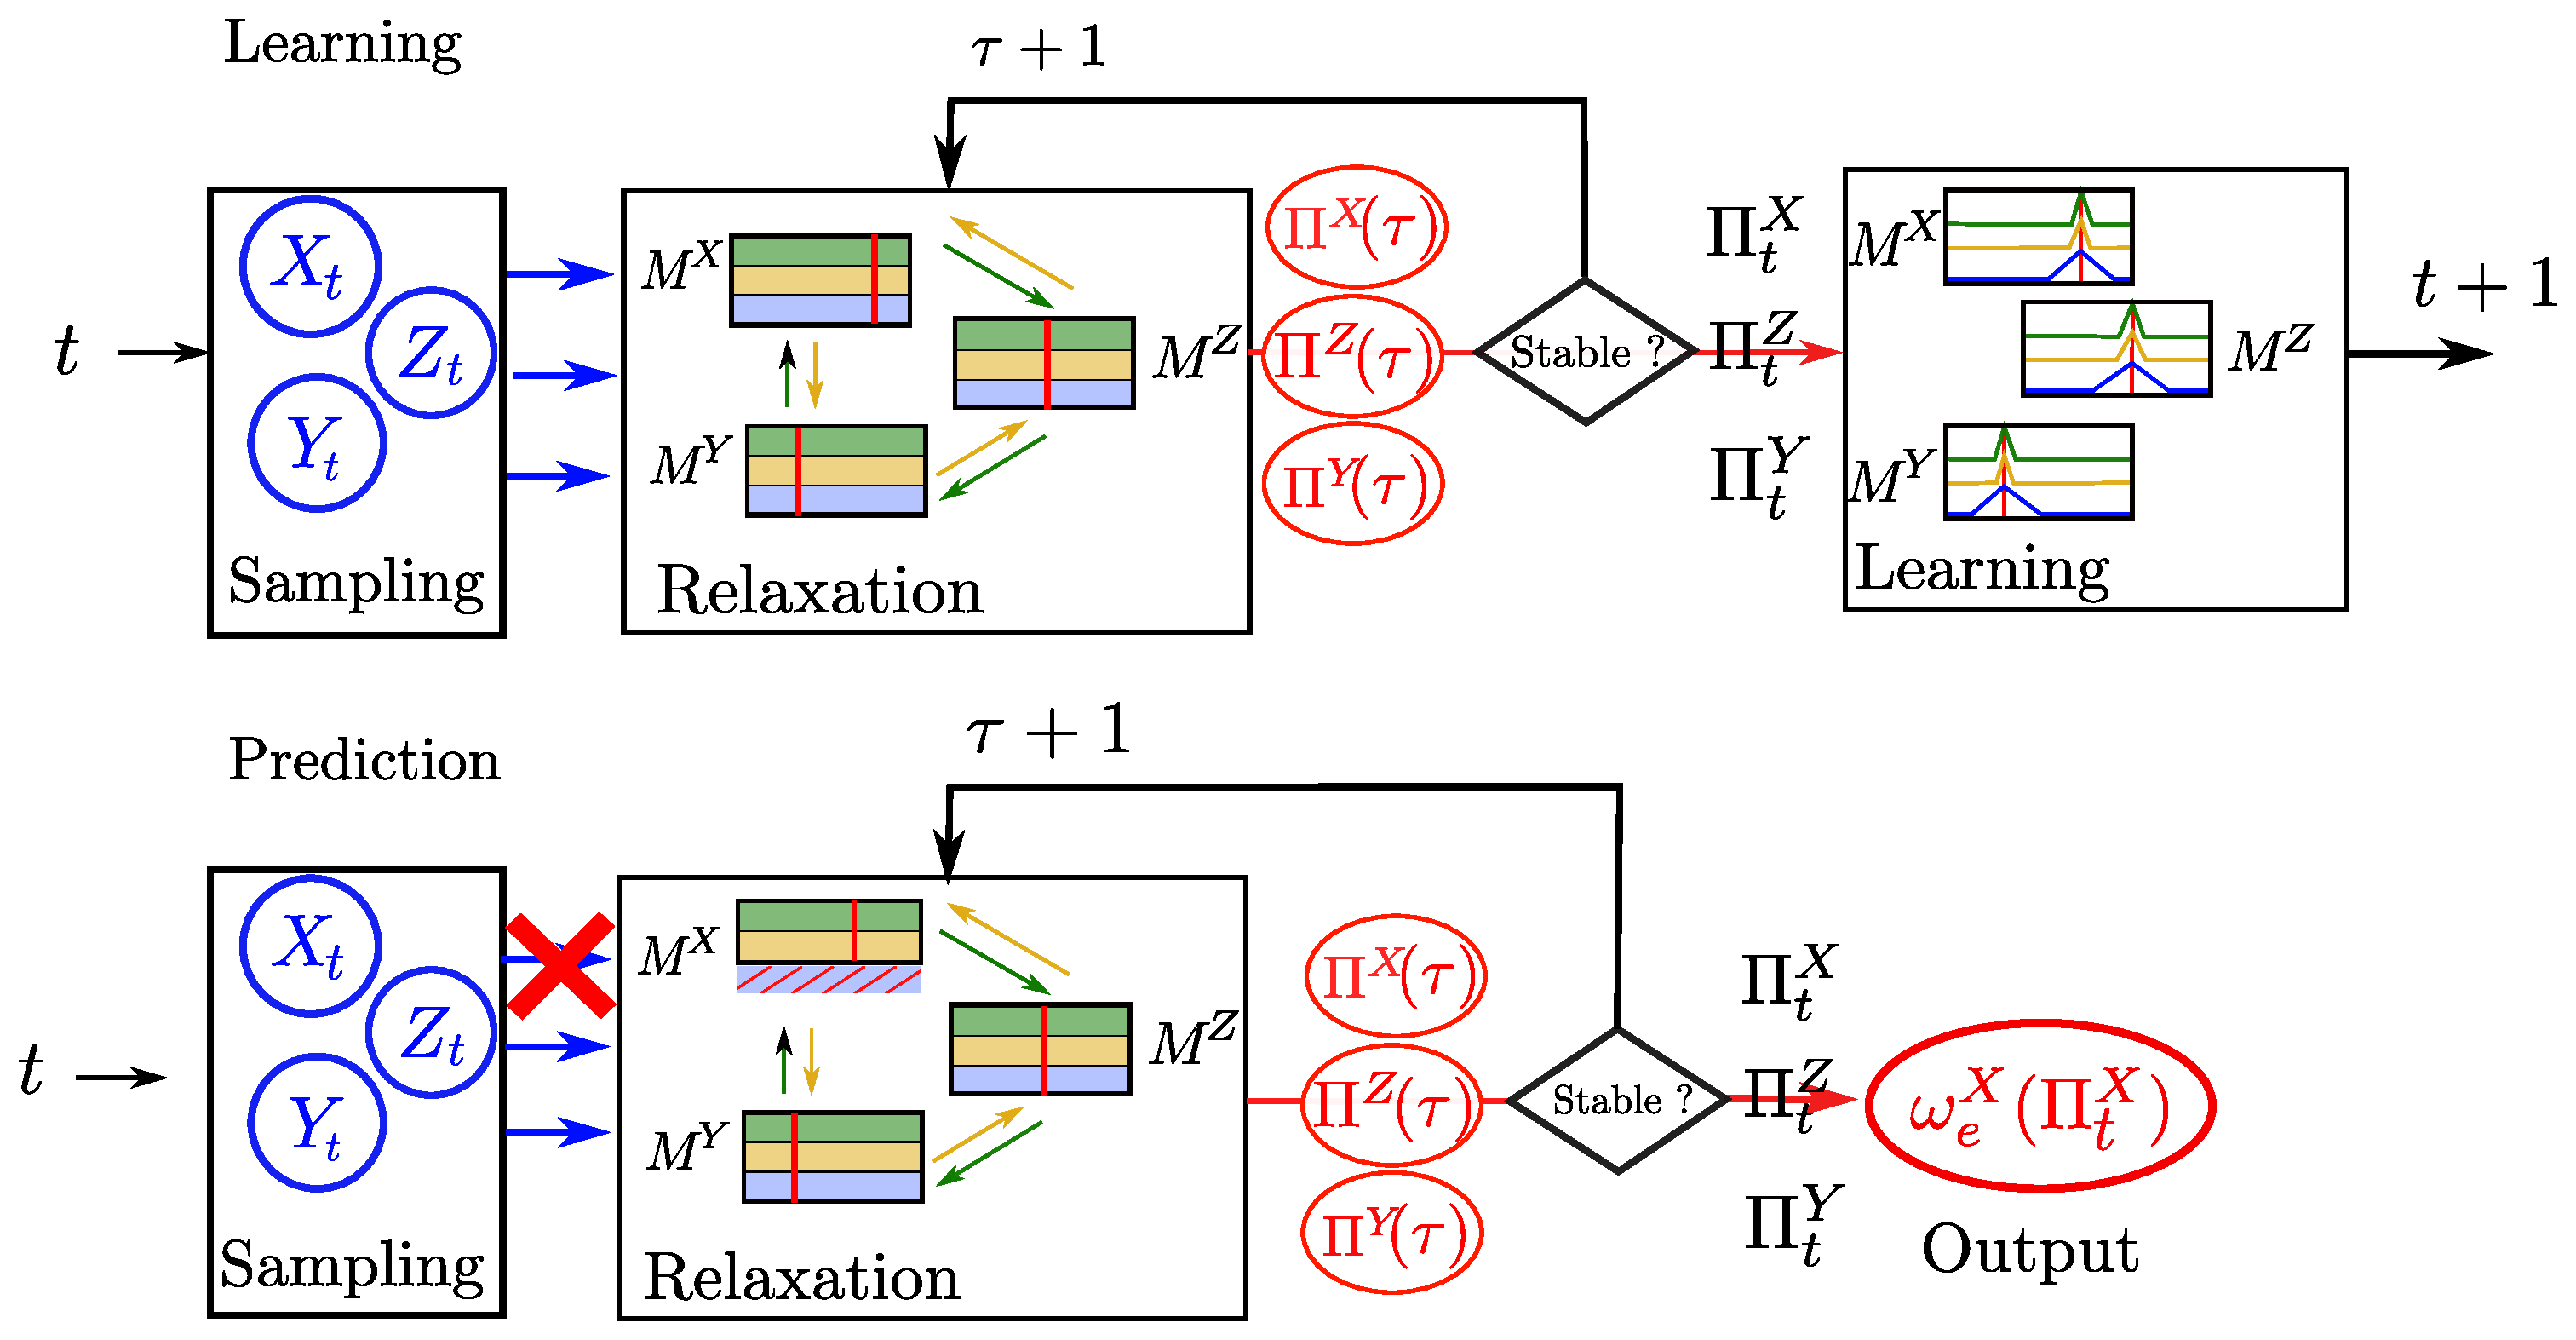
\includegraphics[width=\textwidth]{learning_tests.pdf}
	\caption{Schéma descriptif des opérations effectuées lors de l'apprentissage et de la phase de prédiction.\label{fig:schema_pred}}
\end{figure}


\subsection{Prédiction d'entrées géométriques}

Nous testons d'abord la qualité de la prédiction sur des dispositions d'entrées géométriques.
Pour qu'une carte puisse faire une prédiction correcte, nous choisissons des entrées telles que la connaissance des entrées et du modèle permet de prédire l'entrée manquante.

Nous prendrons ainsi des entrées disposées sur un cercle en deux dimensions plongé et pivoté dans l'espace en 3D \ref{fig:cercle3}. De cette manière, la connaissance de deux des trois coordonnées permet de déterminer la troisième avec précision. Nous testerons également la prédiction d'entrée sur un plan 2D pivoté en trois dimensions.

Ces tâches de prédictions sont réalisées sur un architecture de trois cartes 1D, toutes connectées entre elles. Chaque carte prend donc deux entrées contextuelles et de ce fait possède deux couches contextuelles.
Nous étendrons la capacité de prédiction aux cartes deux dimensions au chapitre suivant.

\begin{figure}
	\centering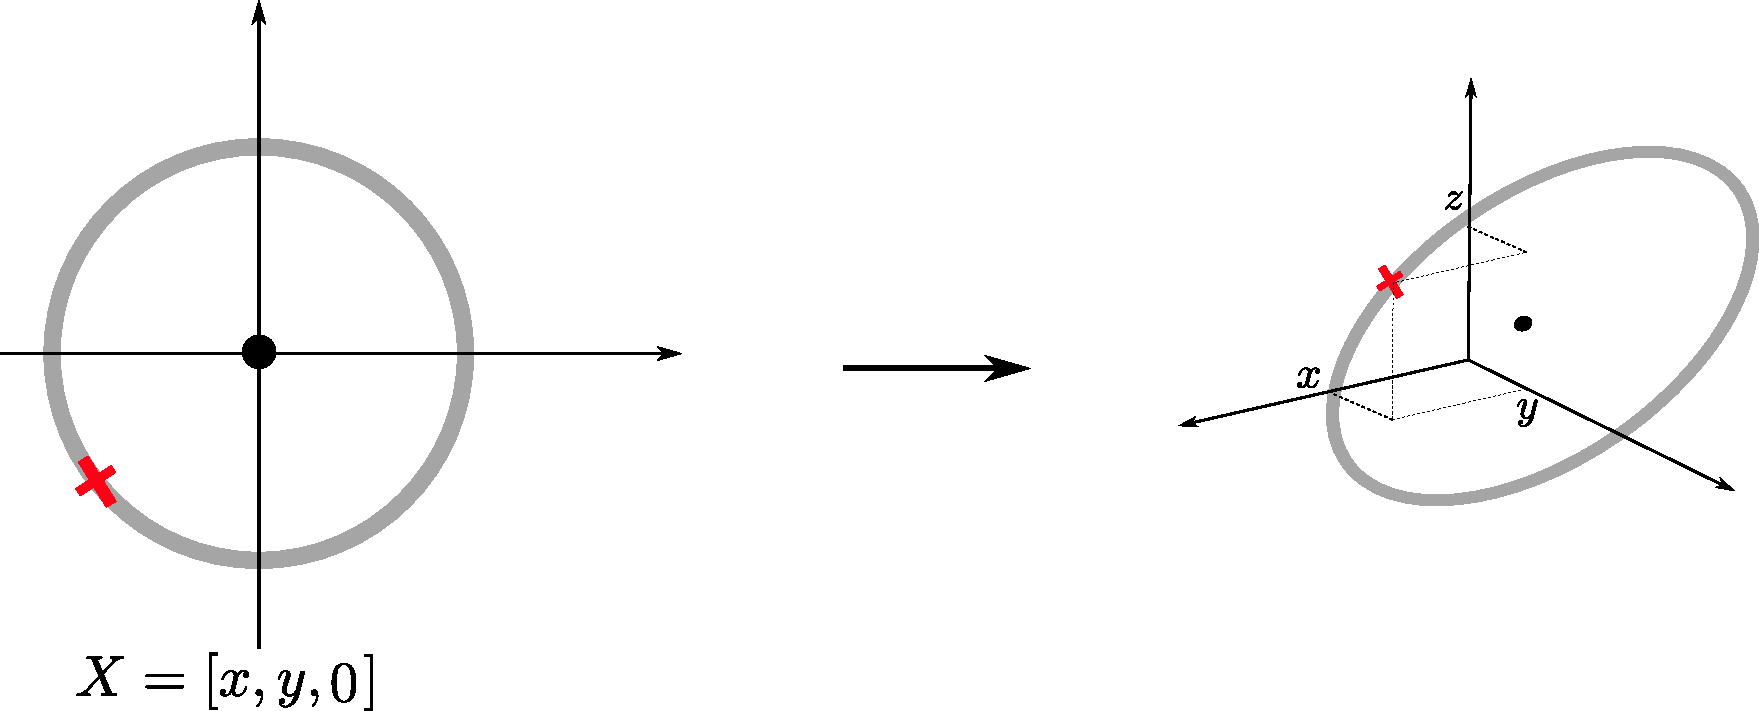
\includegraphics[width=0.9\textwidth]{anneau_inputs.pdf}
	\caption{Exemple de courbe plongée en trois dimensions. La figure 2D est pivotée en trois dimensions. Chaque coordonnée est normalisée de façon à s'étendre entre 0 et 1 en trois dimensions.
	\label{fig:in_3D}}
\end{figure}

La figure \ref{fig:w_cercle} présente la disposition des poids des trois cartes de l'architecture après apprentissage ainsi que des entrées associées. 
Comme dans la version à deux cartes, les poids contextuels s'organisent en plusieurs zones au sein desquelles la valeur de $U$ est située dans une même plage de valeur. 
La figure \ref{fig:pred_cercle} présente ensuite l'erreur obtenue lors de la phase de prédiction. L'entrée $X\m{1}$ n'est ici pas présentée à la carte et sa valeur est prédite par $\w\ext\m{1}{\bmu\m{1}}$. 
Cette figure nous montre que la prédiction est correctement réalisée par l'architecture de cartes. Remarquons que la disposition de l'erreur en lignes horizontales correspond aux zones définies par les valeurs des poids contextuels d'une carte.

Nous traçons également en Figure~\ref{fig:plan3} la disposition des cartes et l'erreur de prédiction obtenue pour des entrées située sur un plan 2D de l'espace en trois dimensions. Ici encore, La connaissance de $X\m{2}$ et $X\m{3}$ définit bien une seule valeur possible de $X\m{1}$. La prédiction est bien réalisée, en remarquant une erreur assez élevée. Nous avons vu que les poids externes des cartes s'étalaient sur le plan en discrétisant l'espace en une centaine de points seulement, bien que chaque carte soit de taille 500 (Voir Figure~\ref{fig:2som_p_d}). Cette discrétisation se retrouve dans l'erreur de prédiction pour trois cartes.

Cette capacité de prédiction est peu précise. Cependant, aucune autre architecture de cartes nous apparaît comme capable de telles tâches de prédiction et prise de décision auto-organisée.


% La figure \ref{fig:w_lissa} présente la disposition des poids sur une courbe de lissajous.
\begin{figure}
	\centering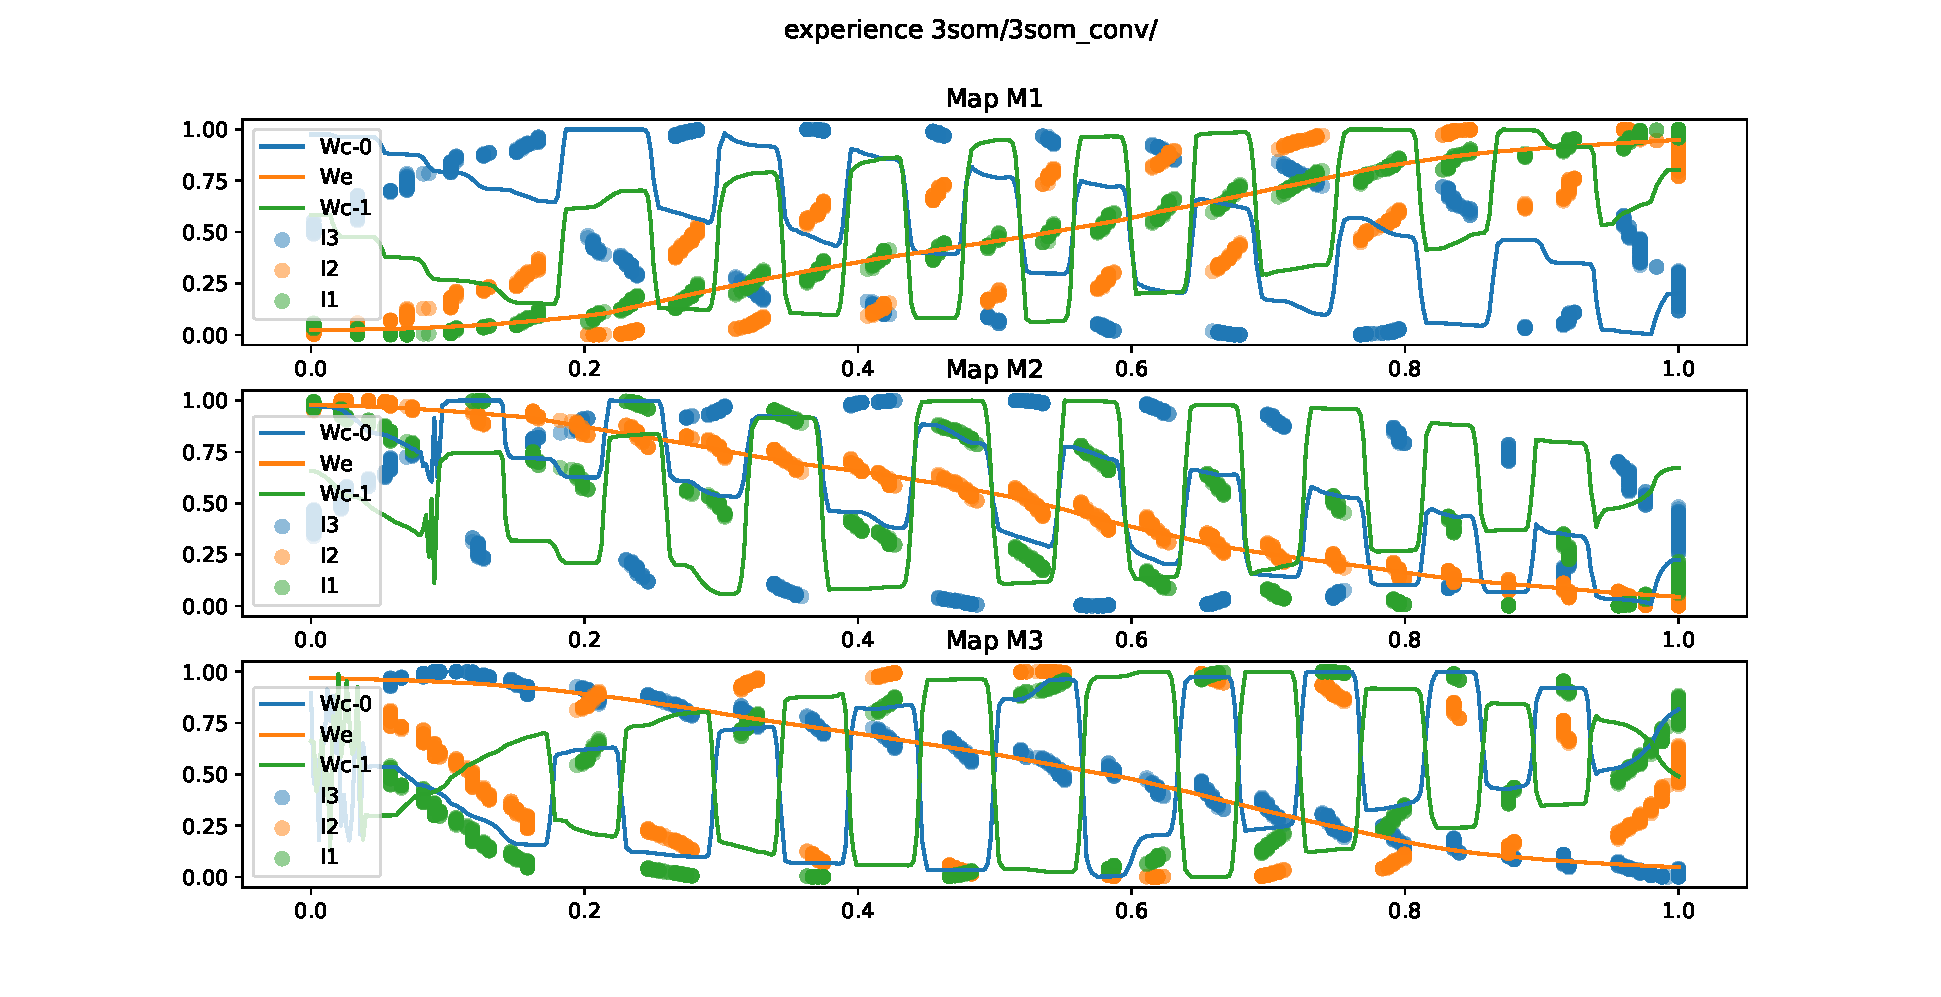
\includegraphics[width=0.9\textwidth]{3som_cercle_w.pdf}
	\caption{\label{fig:w_cercle}}
\end{figure}
% \begin{figure}
% 	\centering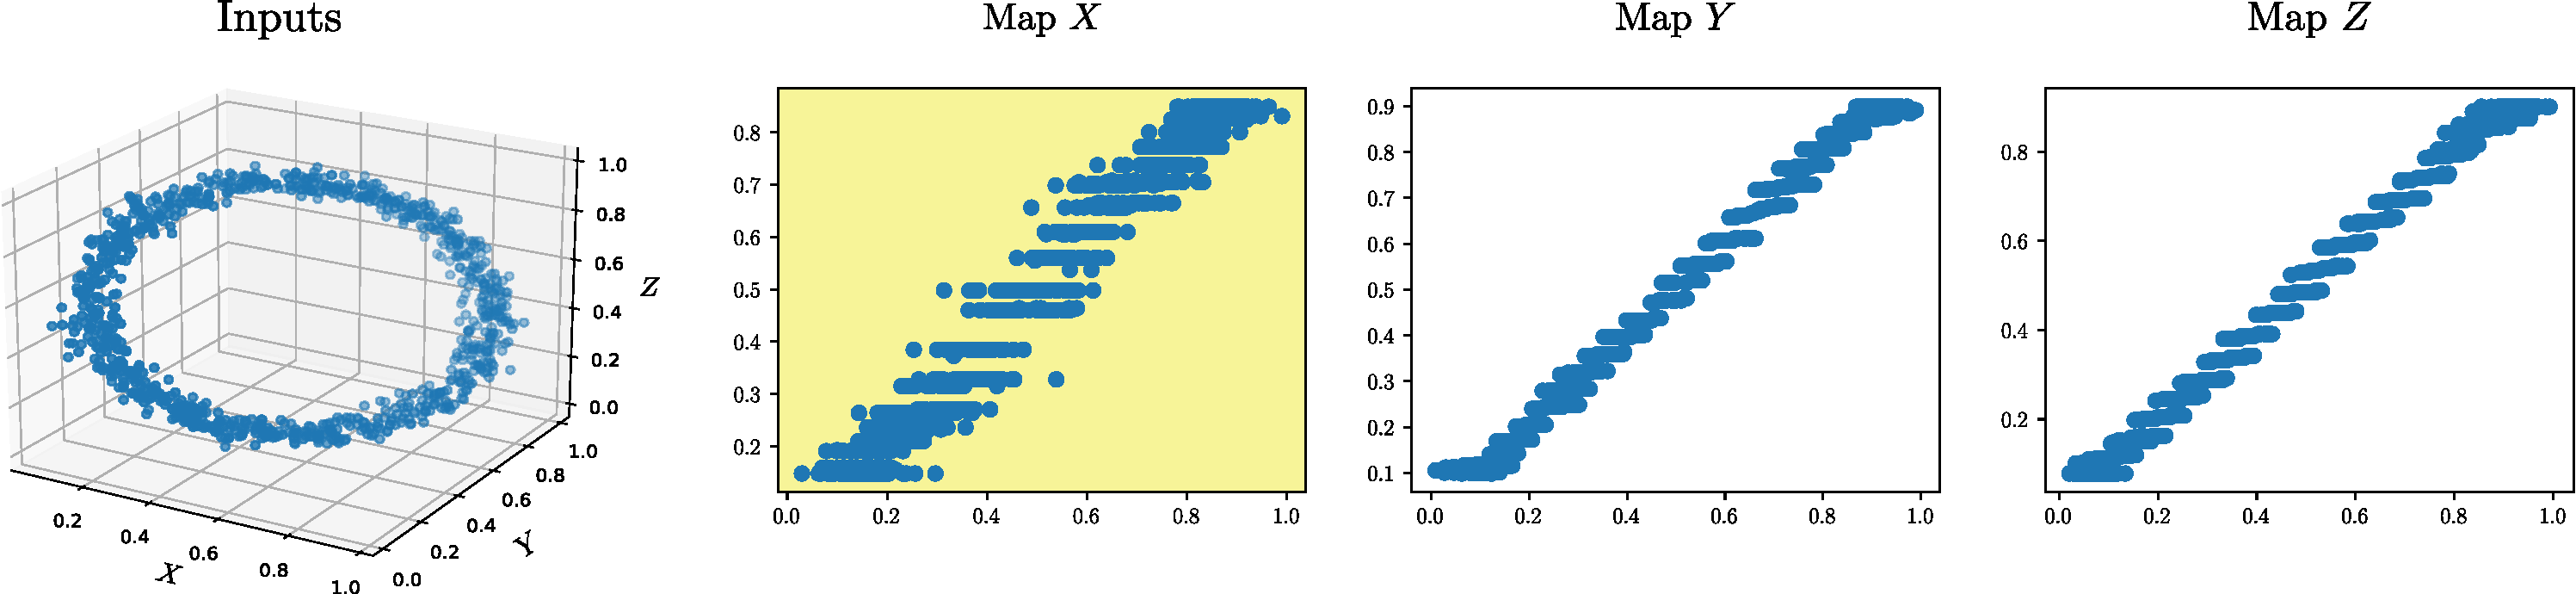
\includegraphics[width=0.9\textwidth]{pred_anneau005_inputs.pdf}
% 	\caption{\label{fig:pred_anneau}}
% \end{figure}

\begin{figure}
	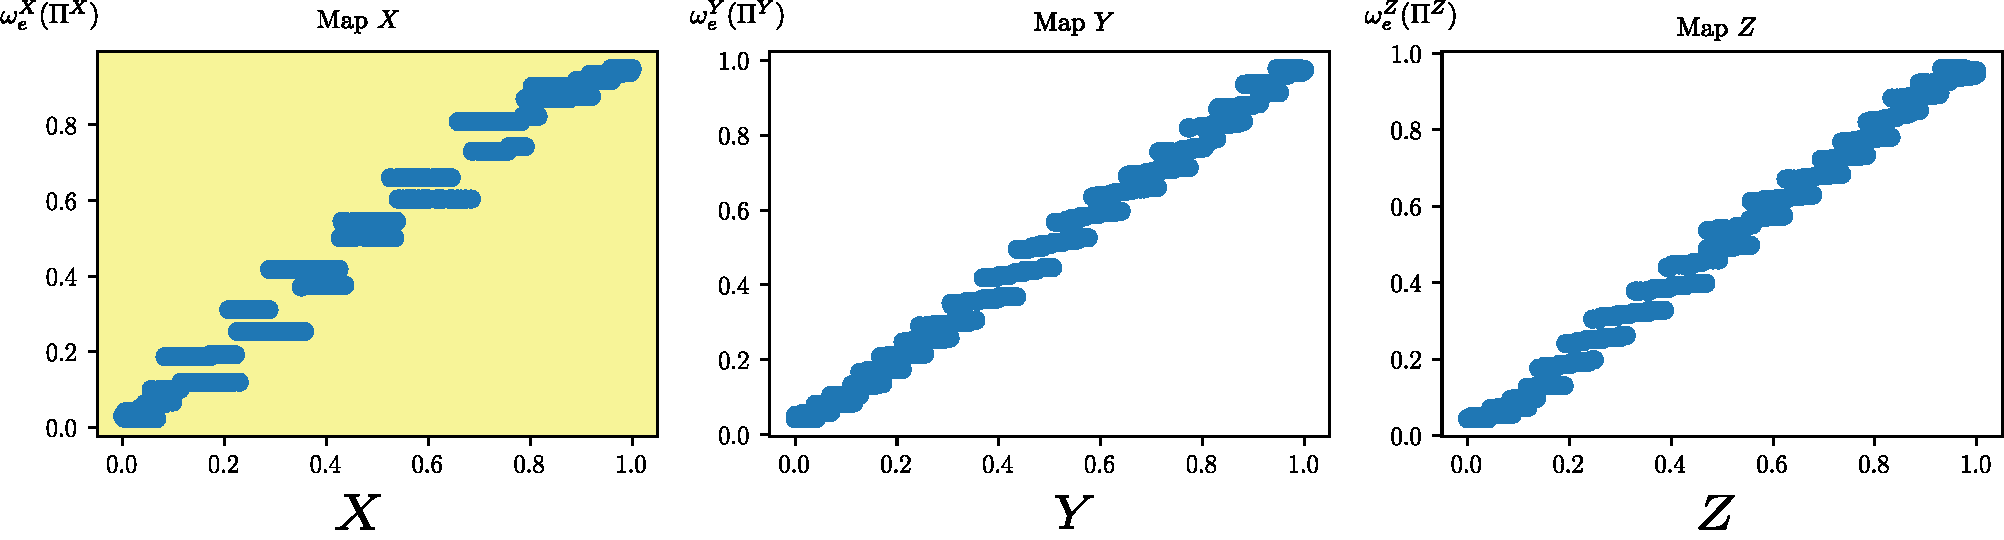
\includegraphics[width=0.9\textwidth]{prediction_x2.pdf}
	\caption{\label{fig:pred_cercle}}
\end{figure}

% \begin{figure}
% 	\centering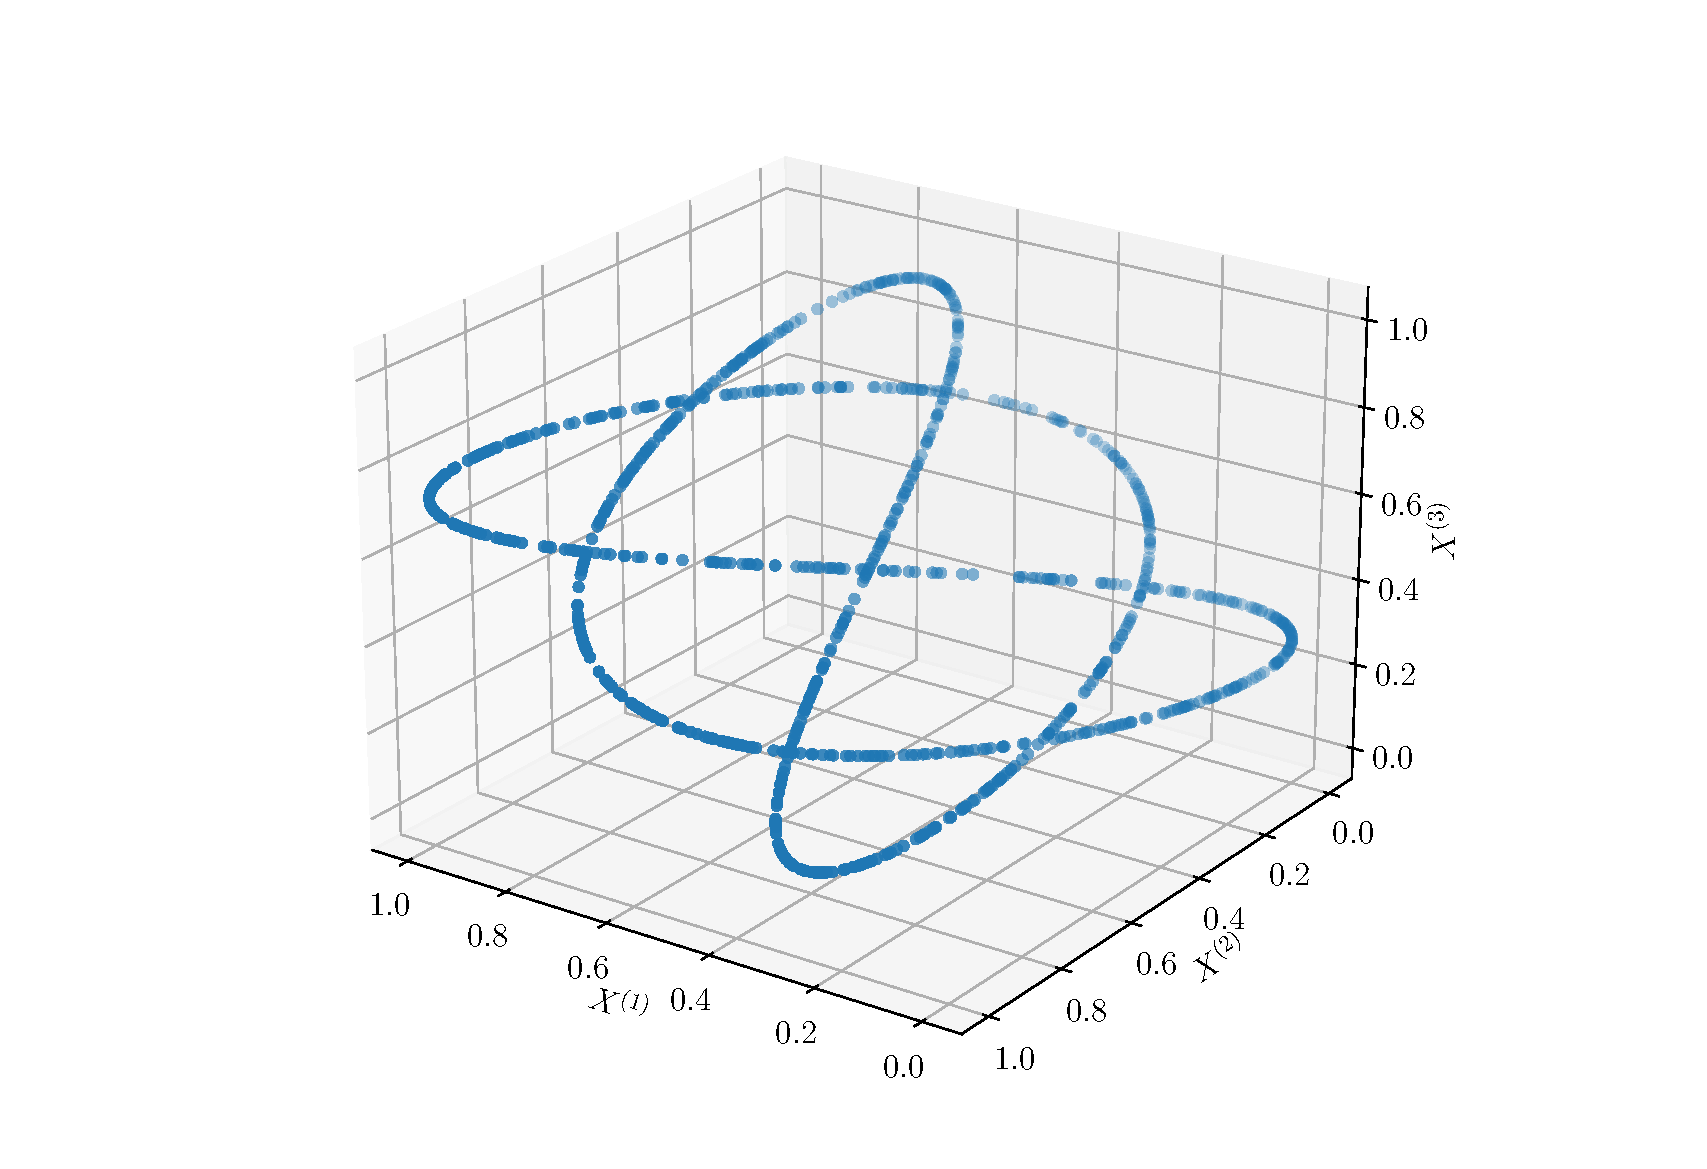
\includegraphics[width=0.5\textwidth]{lissa3D/inputs_lissa}
% 	\caption{Disposition des entrées sur une courbe de lissajous pivotée sur trois dimensions. Étant donné que la courbe est inscrite dans un plan, la connaissance de deux entrées est suffisante pour déterminer la troisième à partir du modèle.\label{fig:in_lissa_3D}}
% \end{figure}

% \begin{figure}
% \begin{minipage}{0.48\textwidth}
% \centering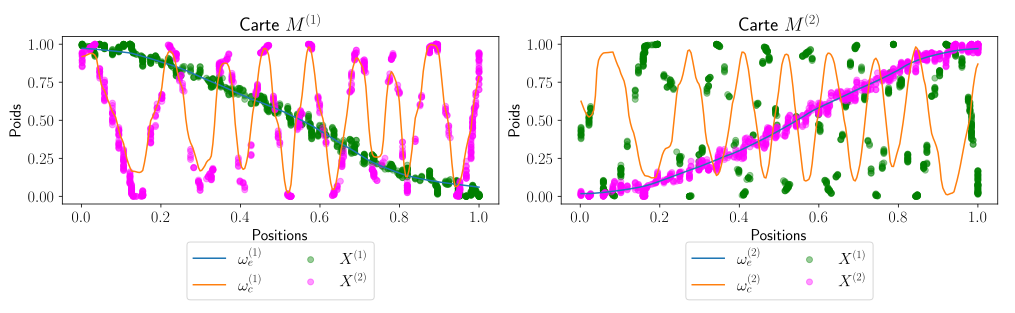
\includegraphics[width=\textwidth]{lissa3D/weights_19999}
% \end{minipage}
% \begin{minipage}{0.48\textwidth}
% \includegraphics[width=\textwidth]{lissa3D/zclosed-1-19999_error}	
% \end{minipage}	
% \caption{Représentation cartographique des poids et entrées des trois cartes après apprentissage d'une courbe de lissajous}
% \end{figure}

\begin{figure}
	\begin{minipage}{0.48\textwidth}
	\centering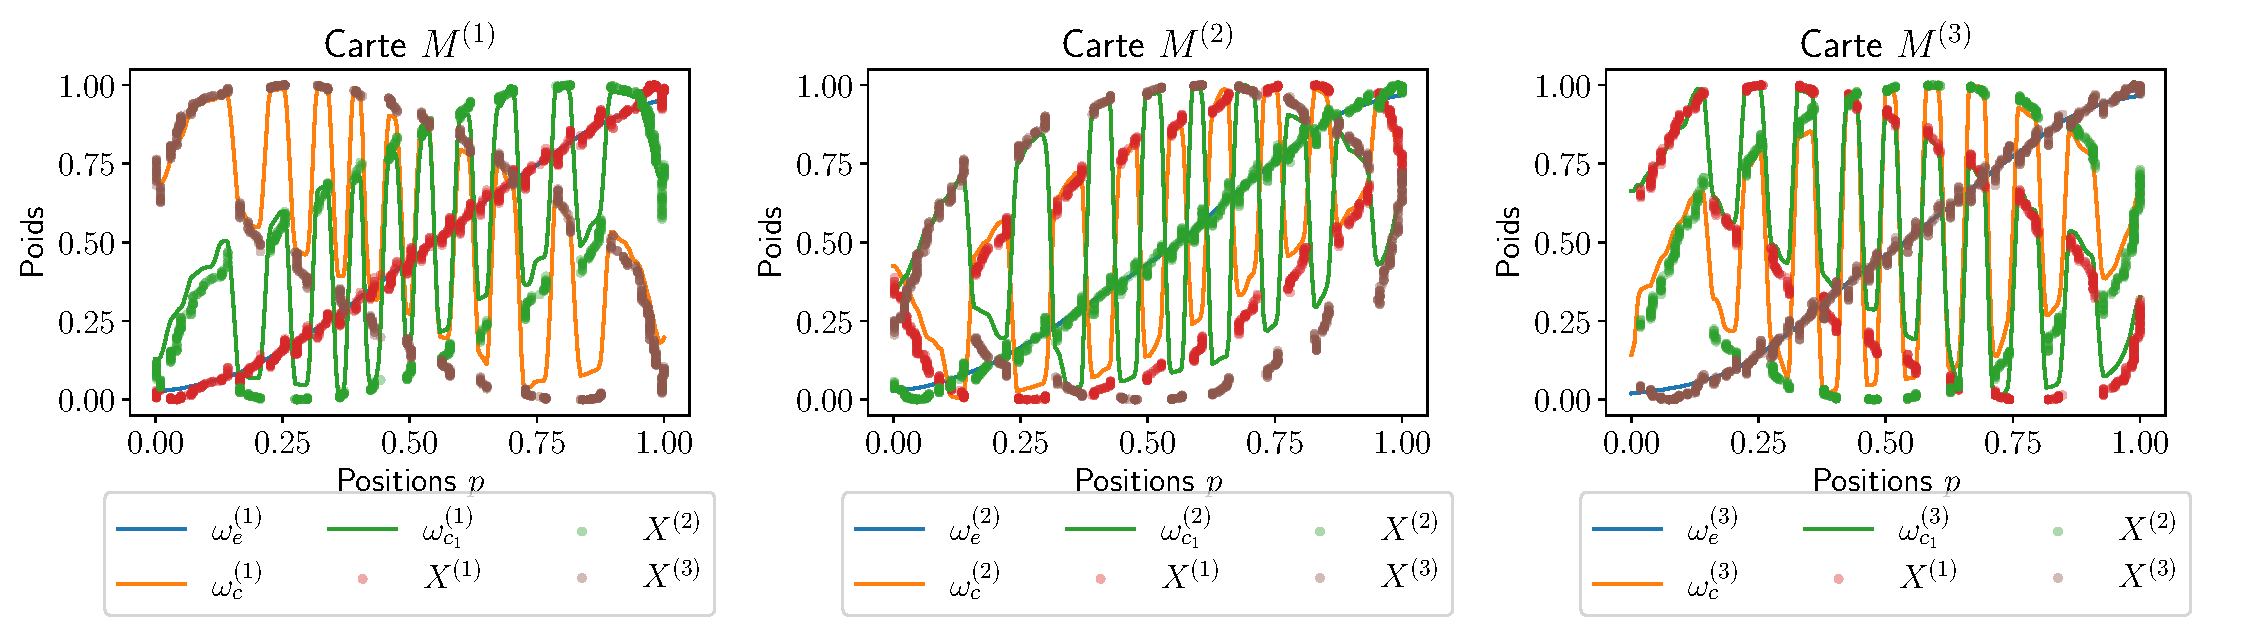
\includegraphics[width=\textwidth]{plan/weights}
	\end{minipage}
	\begin{minipage}{0.48\textwidth}
	\includegraphics[width=\textwidth]{plan/zclosed-1-19999_error}	
	\end{minipage}	
	\caption{Représentation cartographique des poids et entrées des trois cartes après apprentissage d'un plan pivoté en 3D \label{fig:plan3}}
	\end{figure}


\subsection{Entrées réelles~: application sur un drône}

Nous sortons du cadre des entrées simulées pour nous placer dans un cas de contrôle réel. 
Nous disposons d'un drône quadricoptère, commandé à distance. Ce drône possède une caméra frontale ainsi qu'un ensemble de capteurs internes. Chacun de ces capteurs peut être considéré comme une modalité d'un espace multimodal. \'A ces modalités s'ajoute la modalité correspondant à la commande envoyée au drône.
Le principe est d'apprendre, à l'aide d'une architecture de cartes, les relations existant entre les modalités des capteurs et de la commande afin d'ensuite prédire la commande à envoyer à partir des capteurs.
Afin que les relations entre la commande et les capteurs soient significatives, nous nous plaçons dans un cas d'application particulier~: le drône vole dans un couloir étroit, en ligne droite. Le but du drône est alors de voler en avant dans le couloir, sans toucher les murs.
Le but de cette expérience est de démontrer la tâche de prédiction en situation réelle. Nous évaluerons ainsi la robustesse de l'algorithme à des données bruitées et la capacité de CxSOM à réagir en temps réel malgré la relaxation.

\subsubsection{Méthode expérimentale}

Le drône utilisé pour l'expérience est un quadricoptère. Il possède une caméra frontale.
Nous le contrôlons à distance par un ordinateur~; la commande est réalisée en envoyant l'accélération angulaire du drône autour de ses trois axes de rotation.
Nous avons accès aux données des capteurs internes, notamment la vitesse linéaire courante selon chaque axe de déplacement.

Dans le cadre de l'expérience, nous extrayons deux éléments visuels spécifiques au couloir à partir de la caméra du drône~: l'abscisse du point de fuite du couloir $x$. Nous calculons également la différence entre les angles du couloir, notée $\varphi$. Ces valeurs sont illustrées en figure~\ref{fig:drone}.
Le drône se déplace dans un couloir étroit, à hauteur constante et vitesse constante.
La commande générant le déplacement en avant (tangage) est maintenue constante. Les commandes permettant le déplacement en largeur sont alors $\omega$ et $\rho$. Dans le cadre de cette expérience, nous contrôlerons uniquement $\rho$.
Enfin, la vitesse linéaire en largeur du drône peut être récupérée à chaque instant~; nous la notons $v$.
Nous avons ainsi quatres modalités lors du déplacement du drône: $x$, $\varphi$, $\rho$ et $v$.
Nous construisons une architecture CxSOM sur ces quatres modalités, composée de quatre cartes connectées chacune aux trois autres.
Une phase d'apprentissage est réalisée sur des déplacements du drône contrôlés humainement. Lors de cette phase, nous avons utilisé un système de contrôle PID pour assister la commande humaine. 
Cette phase d'apprentissage est réalisée hors ligne pour que les données soient présentées aléatoirement aléatoirement lors de l'apprentissage.
Après apprentissage, nous effectuons une phase de prédiction. Lors de cette étape, la commande $\rho$ n'est plus présentée à la carte correspondante. Nous envoyons alors le poids externe du BMU de cette carte comme commande du drône. Cette étape est réalisée en ligne, sur des trajectoires réelles du drône.

La figure \ref{fig:drone_inp} présente la répartition des entrées présentées au drône. Nous avons tracé les dépendances entre chaque modalité. Nous remarquons sur la figure qu'une dépendance forte se dégage entre les entrées ?? et ??, ainsi que ?? et ??. Si les cartes apprennent correctement le modèle liant les entrées, la prédiction peut être réalisée.
Ces dépendances sont très bruitées. Cette expérience en conditions réelles nous permettra d'observer la résistance au bruit de la prédiction.

%TODO mettre disposition des entrées.

\subsubsection{Résultats}
La carte associée à $\rho$ possède donc une couche de poids externe et trois couches de poids contextuels. Ces poids sont représentés en figure \ref{fig:drone_w}. L'organisation des poids contextuels rappelle celle observé dans des conditions géométriques: les poids contextuels définissent des zones. Contrairement à l'expérience réalisée sur un cercle, la taille de ces zones dépend de la couche de poids contextuel définie. 

\begin{figure}
\begin{minipage}{0.5\textwidth}
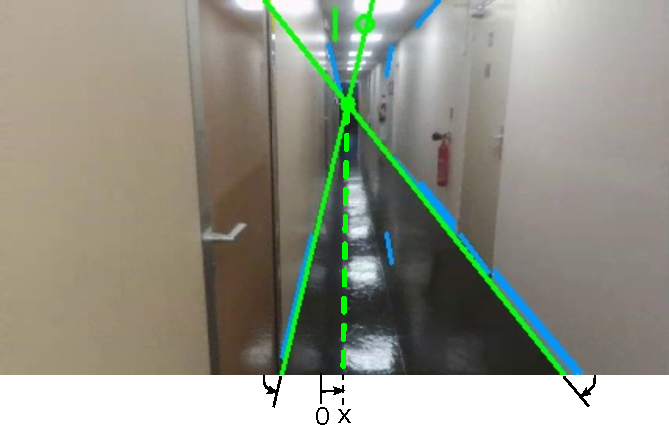
\includegraphics[width=\textwidth]{visudrone}
\end{minipage}
\begin{minipage}{0.5\textwidth}
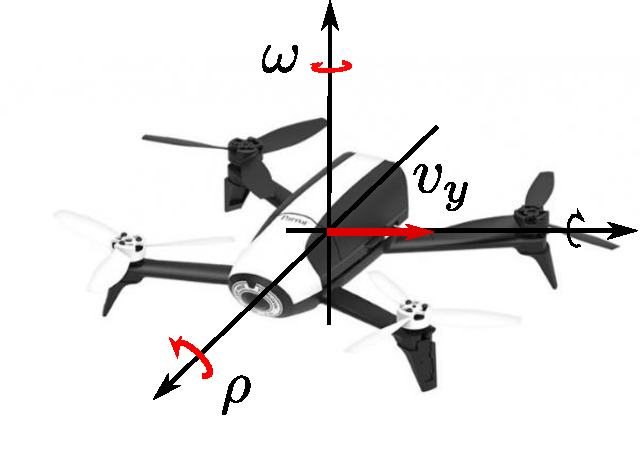
\includegraphics[width=\textwidth]{dronesteup}
\end{minipage}
\caption{Disposition des capteurs utilisés pour l'expérience}
\label{fig:drone}
\end{figure}

\begin{figure}
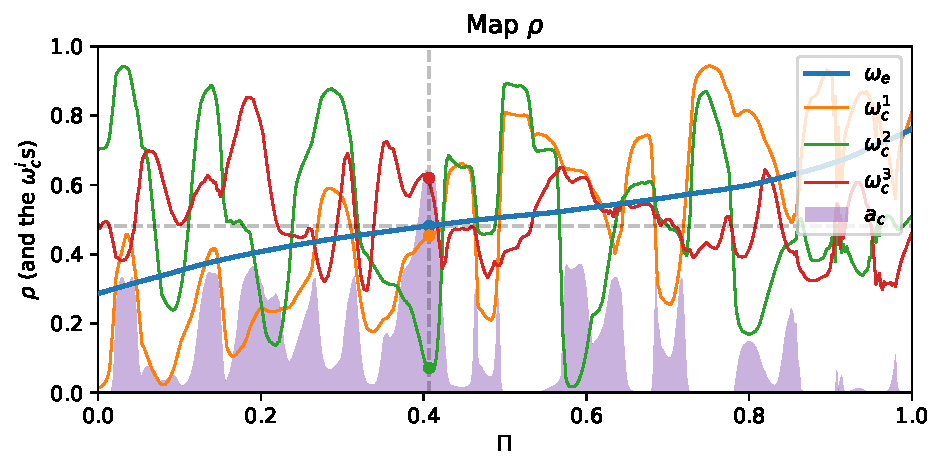
\includegraphics[width=\textwidth]{dronemap}
\caption{Disposition des poids de la carte $\rho$ après apprentissage et exemple de calcul d'activité}
\label{fig:drone_w}
\end{figure}

\subsubsection{Discussion}
Ici on ne cherchait pas à comparer avec des valeurs théorique, mais on observe que le drone ne tape pas les murs
Illustration de la capacité de prédiction et mémoire associative
Resistance au bruit

Calcul des dépendance entre les entrées et la commande:
PCA sur les entrées, calcul de MI après apprentissage

\section{Conclusion}


\ifSubfilesClassLoaded{
    \printbibliography
    %\externaldocument{../main.tex}   
}{}
\end{document}